% !TeX spellcheck = en_US
\documentclass[12pt, a4paper, titlepage]{book}
%\usepackage[a4paper, margin=3cm]{geometry}
%\usepackage{setspace}
%\setstretch{1.5}

\usepackage[utf8]{inputenc}% erm\"oglich die direkte Eingabe der Umlaute 
\usepackage[T1]{fontenc} % das Trennen der Umlaute
\usepackage[english]{babel}
\usepackage[breaklinks,hidelinks]{hyperref}
\usepackage{xspace}
\usepackage{lmodern}
\usepackage{textcomp}
\usepackage{graphicx}
\usepackage{color}
\usepackage{caption}
\usepackage{comment} 
\usepackage{float}
\usepackage{listings}
\usepackage{csvsimple}
\usepackage{longtable}

\usepackage{amssymb}
\usepackage{amsmath}

\usepackage[square,comma]{natbib}
\usepackage[titletoc]{appendix}

% set date format
\usepackage[style=iso]{datetime2}
%\usepackage[yyyymmdd]{datetime}
%\renewcommand{\dateseparator}{--}

% shortcuts
\newcommand{\jws}{JWS~Online\xspace}
\newcommand{\django}{Django\xspace}
\newcommand{\sedml}{SED-ML\xspace}
\newcommand{\mathml}{MathML\xspace}
\newcommand{\simexp}{simulation experiment\xspace}
\newcommand{\fairdom}{Fairdom\xspace}
\newcommand{\mathematica}{Mathematica\xspace}
\newcommand{\json}{JSON\xspace}
\newcommand{\numl}{NuML\xspace}
\newcommand{\combine}{COMBINE\xspace}
\newcommand{\ca}{\combine~archive\xspace}
\newcommand{\sbml}{SBML\xspace}
\newcommand{\cellml}{CellML\xspace}
\newcommand{\xml}{XML\xspace}
\newcommand{\rdf}{\xml~RDF\xspace}
\newcommand{\owl}{OWL\xspace}

\newcommand{\masymos}{MaSyMoS\xspace}
\newcommand{\bives}{BiVeS\xspace}
\newcommand{\comodi}{COMODI\xspace}
\newcommand{\neoj}{neo4j\xspace}

\newcommand{\sysbio}{Systems Biology\xspace}
\newcommand{\rest}{REST\xspace}  % like in REST interface

% TODO command
\newcommand{\todo}[1]{{\color{red} TODO: #1}\\}
\newcommand{\dw}[1]{\textbf{\color{green} DW: #1}\\}

\title{Conception and Prototypic Implementation of a Storage Solution for Models with Multiple Versions}
\author{Martin Peters\\[12pt]
	\small Department of Systems Biology and Bioinformatics\\
	\small University of Rostock}
\date{\today}

\begin{document}
	%title
	\maketitle
	% info about compiling date
	\pagebreak
	~ \vfill
	{\hfill \tiny \LaTeX ~compiled at \DTMnow}
	\pagebreak
	% the toc
	\tableofcontents
	
	% set paragraph indents
	%\setlength{\parindent}{0pt}
	%\setlength{\parskip}{12pt plus 0mm minus 3mm}
	
	\chapter{Introduction}
	% comment command for Dagmar (defined in shortcuts.tex)
	%\dw{This a is comment from Dagmar}
	% !TeX spellcheck = en_US
%\section{Motivation}
"Scientific publications have at least two goals: (i) to announce a result and (ii) to convince readers that the result is correct" \citep{Mesirov2010}.
This paradigm has ruled the world of scientific publications since its beginnings, but the last two decades proved to provide challenges for it. With the improvement and further development of computational tools, more advanced analysis and complex computation methods are available to a broader audience by software packages and tools. Now, people who have no or very little background in Mathematics or Computer Science face the challenge to comply with the second point mentioned by \citeauthor{Mesirov2010}. Also with increasing complexity it becomes challenging to describe the complicated workflow within the word limitation of a normal publication.
For instance, biologists can now easily acquire large DNA or RNA sequencing datasets, which  are too large to analyze manually.
This data first needs to be preprocessed in order to extract meaningful results. %Those data needs to be sanitized, converted and condensed, to make sense out of it.
Very often researchers without a computer science background do not accurately describe their methodology, hence resulting findings can not accurately be reproduced \citep{Peng2011}.
%Resulting publications often only pay little attention to the computational processes involved or even to the used algorithms \citep{Peng2011}.
Since the work cannot be reproduced, it is not possible to build upon the findings and therefore the hypothesis cannot be proven.
%But why is it of such a tremendous importance to know exactly every step leading to a result? Basically this is the foundation of scientific publications and peer review. Without in-depth knowledge of the methods, the environment and the workflow it is impossible to reproduce the experiment or observation and therefore it is impossible to prove or disprove the correctness of the assumption. 
%This inability may lead into blind trust in publications, making room for wrong or made-up scientific findings.
Especially valuable are these reproduction information, when dealing with studies, which may not be easily independently redone, because of resource, time or financial constraints \citep{Peng2011}.
\todo{Provide the example from the Peng? guy.} \todo{emphasis one of the constraints in the expample -> time}
Therefore ways or methods of reproducibility need to be widely addressed. \citeauthor{Mesirov2010} suggests researchers to make use of a Reproducible Research Environment, providing a set of tools "with the ability to automatically track the provenance of data, analyses, and results and to package them" \citep{Mesirov2010}.

\sysbio is an interdisciplinary field that heavily relies on people with different academic backgrounds, it is therefore especially important to ensure the clear reproducibility and exchangebility of data.
Models are a condensed way to represent knowledge and data and are essential to \sysbio.
Due to the importance of models in \sysbio, it is imperative that they are reproducible and built using standard formats \citep{Drager2014}.
It is of great importance to use standard formats because tools used to create the original model may no longer be available or supported \citep{Peng2011}.
\todo{That is, when a model is encoded in standard formats, the possibility of at least one tool able to decode this format in future is higher.}
Furthermore, standardization and reproducibility are needed in order expand on and share existing findings.
To this extend the \combine initiative has been founded to "coordinate the development of the various community standards and formats for computational models" \citep{COMBINE}.
Even though a standard to describe biological networks was successful, it was not sufficient in terms of the goal to ensure reproducibility. Therefore, \citeauthor{Waltemath2011a} developed \sedml \citep{Waltemath2011a} to share simulation experiment setups automating the workflow of creating, sanitizing, converting, condensing, and plotting data.

In addition to \sedml, the \ca was introduced by \citet{Bergmann2014a} such as to share relevant information and data regarding reproduction. This standard is useful and important for sharing additional information \citep{Bergmann2014a}. % such as basic provenance information.
Despite the benefits of using the \ca, certain problems have arisen. For instance, a \ca is a snapshot of a complex development process. It can only ship one specific version and no references to older or newer versions are available. This is indeed desired when reproducing specific findings from a model used in a publication, but however hinders the incorporation of newer versions of models or simulation descriptions to the already existing (simulation) study.

The lack of the references to older or newer versions creates a lack of transparency, since "users are often not only interested in the current value of data but also in changes" \citep{Cobena2002}. Furthermore there is currently no available model repository that is able to query and compare multiple model versions in a simple manner.
The main goal of this thesis is therefore to investigate a concept to store biological models in such a way that multiple versions can be accessed, queried, and compared. I furthermore introduced semantical annotations of changes between model versions, by doing so I improved the ability to query for a version of a model by specific criteria. Consequently it will also improve the user experience for systems biologists seeking to build onto existing models, as the evolution of models plays an important role for them \citep{Scharm2015}.

\begin{comment}

\begin{itemize}
\item Why is Reproducibility important (in life science/Bioinformatics)
	\subitem what is a problem?
	\subitem why is it important?
	\subitem specific points regarding Systems Bio
	\subitem refs to reproducible science
	
	\subitem "Scientific publications have at least two goals: (i) to announce a result and (ii) to convince readers that the result is correct. Mathematics papers are expected to contain a proof complete enough to allow knowledgeable readers to fill in any details. Papers in experimental science should describe the results and provide a clear enough protocol to allow successful repetition and extension." \citep{Mesirov2010}
	\subitem "More recently, scientists who are not themselves computational experts are conducting data analysis with a wide range of modular software tools and packages. Users may often combine these tools in unusual or novel ways. In biology, scientists are now routinely able to acquire and explore data sets far beyond the scope of manual analysis, including billions of DNA bases, millions of genotypes, and hundreds of thousands of RNA measurements. Similar issues may arise in other fields, such as astronomy, seismology, and meteorology. While propelling enormous progress, this increasing and sometimes “indirect” use of computation poses new challenges for scientific publication and replication. Large data sets are often analyzed many times, with modifications to the methods and parameters, and sometimes even updates of the data, until the final results are produced. The resulting publication often gives only scant attention to the computational details. Some have suggested these papers are “merely the advertisement of scholarship whereas the computer programs, input data, parameter values, etc. embody the scholarship itself ” (2). However, the actual code or software “mashup” that gave rise to the final analysis may be lost or unrecoverable." \citep{Mesirov2010}
	\subitem "The first element is a Reproducible Research Environment (RRE) for doing the computational work. An RRE provides computational tools together with the ability to automatically track the provenance of data, analyses, and results and to package them (or pointers to persistent versions of them) for redistribution." \citep{Mesirov2010}
\item Reproducibility
	\subitem \sedml scripts fails, when model changes
	\subitem cf. (Casadevall and Fang, 2010; Gentleman, 2005; Laine et al., 2007; Mesirov, 2010; Peng, 2011; Sandve et al., 2013; Waltemath et al., 2011, 2013b) \\ refs shameless stolen from bives paper discussion section
	\subitem " Researchers across a range of computational science disciplines have been calling for reproducibility, or reproducible research, as an attainable minimum standard for assessing the value of scientific claims, particularly when full independent replication of a study is not feasible (4–8)." \citep{Peng2011}
	\subitem "A critical barrier to reproducibility in many cases is that the computer code is no longer available. Interactive software systems often used for exploratory data analysis typically do not keep track of users’ actions in any concrete form. Even if researchers use software that is run by written code, often multiple packages are used, and the code that combines the different results together is not saved (10). Addressing this problem will require either changing the behavior of the software systems themselves or getting researchers to use other software systems that are more amenable to reproducibility." \citep{Peng2011}
	\subitem "[...] reproducibility is critical to tracking down the “bugs” of computational science. In cases with interesting findings, reproducibility can 	greatly facilitate building on those findings (12)." \citep{Peng2011}
	

\item Transparency
	\subitem "Tracking the evolution of a model, that is providing information about changes in the model and its encoding, plays an important role in supporting the user " \citep{Scharm2015}
	\subitem "Users are often not only interested in the current value of data but also in changes." \citep{Cobena2002}
	\subitem "The primary purpose of an archive is not to ensure replicability (King 1995, 494) but to enhance extensibility (which presumes replicability). Thus, an archive should make it easier for one researcher to build on the work of another [...]" \citep{McCullough2008}
	\subitem " For this reason, ‘data only’ archives are not conducive to replication; only data+code archives can facilitate replication. Even when data are proprietary, the code should still be made available, so that other researchers can apply the same method to new data or to check the accuracy of the code. See our recommendation 8 in the appendix." \citep{McCullough2008}
	
\item Tracking differences (Provenance)
	\subitem what has changed
	\subitem who has changed it
	\subitem oxford2012 + first bives paper

\item "distribution of models through these repositories accelerates collaborative research and encourages model reuse" \citep{Scharm2015}

\item Doing analysis of the evolution of a biological model
\item provide a comprehensive repository of biological models and their history
\item discover similarities and differences in the development of model through Ontology crosslinking
\item Motivation out of koehn2008 \citep{Kohn2008}
\end{itemize}

\todo{last paragraph of motivation is goals section, summarizing proposed solution}
\todo{research gap ausarbeiten}
\todo{look into MOST for stats regarding model versions}

\section{Objectives}
\begin{itemize}
\item develop a concept to support different versions in model databases
	\subitem \todo{mention masymos directly?}
	\subitem \todo{arg. structure bives->masymos//masymos->bives//generische mdb->version concept->bives->goal}
\item semantically connect the versions
	\subitem relation between versions? + comodi terms
	\subitem ref to semantic web
	\subitem reason -> allow evaluation and analysis
\item store differences to allow for efficient analysis
\item \todo{talk about possible results}
\end{itemize}
\end{comment}
	
	\chapter{Difference detection and its challenges for Systems Biology Models}
	\chaptermark{Difference detection}
	% !TeX spellcheck = en_US
\section{Data formats for System Biology models}
	\label{sec:background:formats}
	\begin{itemize}
		\item formats
		\subitem SBML
		\subitem CellML
		\subitem \sedml
		\item everything in XML
		\item semantic annotations
	\end{itemize}
	\todo{look at STATS paper/MOST for version statistics}

\section{Detecting differences in Version Control Systems}
	\label{sec:background:diff}
	
	\subsection{Unix Diff}
	\label{sec:background:diff:unix-diff}
	The essential building block for each Version Control System (VCS) is an algorithm or tool to detect differences between two or more version, because just storing each version completely is a waste of storage and bandwidth. Further processing change sets enables the system to automatically merge different development branches and therefore making collaboration more efficient.
	
	Nowadays all general-purpose VCS use the \emph{diff} utility, developed as part of UNIX. It is based on the Hunt-McIlroy algorithm, which tries to solve the longest common subsequence problem for two files \citep{Hunt1976}.
	The result is a report of all differences between two files, "expressed as a minimal list of line changes to bring either file into agreement with the other" \citep{Hunt1976}.
	
	\begin{comment}
	\begin{itemize}
		\item Based on solving the longest common subsequence problem
		\item "The program diff reports differences between two files, expressed as a minimal list of line changes to bring either file into agreement with the other" \citep{Hunt1976}
		\item "The central algorithm of diff solves the ‘longest common subsequence problem’ to find the lines that do not change between files" \citep{Hunt1976}
	\end{itemize}
	\end{comment}
	
	\subsection{XML Diff}
	\label{sec:background:diff:xml-diff}
	The problem with general-purpose VCS or more specific the difference algorithm used by them (cf. section \ref{sec:background:diff:unix-diff}) is, however, that they do not make any or very little assumptions about the underlying document and therefore fail to recognize features, specific to the format. These line-base algorithms proved to be problematic especially for \xml, since line breaks can be neglected, without changing the encoded information. \citep{Ronnau2005}
	
	It can be concluded, that the usual diff algorithm is too fine granular, since it also reacts to changes in the encoding. Generally \xml can be represented as hierarchical tree structure and thus it is possible to detect changes based on their position in the tree, instead by a line-number \citep{Wang2003,Chawathe1996,Cobena2002}.
	This can be archived by identifying unchanged subtrees and map them between source and destination version. Going out from those mapped tree, more and more nodes can be matched, under consideration of ancestors, descendants, and labels. Also changed attributes or text-nodes need to be treated differently \citep{Cobena2002}.
	
	\todo{add ref to both examples XyDiff + the other one?}
	
	\begin{comment}
	cf. Cobena2002 \citep{Cobena2002} and \citep{Waltemath2013} in section 2.2.1
	Chawathe et al., 1996 \citep{Chawathe1996}
	\begin{itemize}
		\item "With flat information deltas may be represented simply as sets of tuples or records inserted into, deleted from, and updated in relations. In hierarchical information, we want to identify changes not just to the 'nodes' in the data, but also to their relationships." \citep{Chawathe1996}
		\item "General-purpose version control systems attempt to handle any kind of document and thus make no assumptions about the underlying document format. Usually, those systems distinguish between binary documents and text documents. Appropriate diff algorithms are employed to detect changes between two versions of a document. Those diff algorithms are either line based (for text documents) or byte based (for binary documents). General-purpose version control systems provide good control for line-organized text documents such as source code or latex documents. For XML documents, where the organization into lines can be neglected, 2 line-based version control is inappropriate." \citep{Ronnau2005}
		\item requirements
			\subitem "Within a delta, the exact location of the change must be identified." \citep{Ronnau2005}
			\subitem "XML Structure Information. An XML document is generally a hierarchically structured document, and can be represented in a tree structure. However, an XML document has other features that distinguish it from a general labeled tree. X-Diff introduces the	notion of node signature and a new matching between the trees corresponding to the two versions of a 	document. Together, these two features are used to find the minimum-cost matching and generate a minimum-cost edit script that is capable of transforming the original version of the document to the new version." \citep{Wang2003}
			\subitem "Unordered Trees. Since XML documents can be represented as trees, the change detection problem is related to the problem of change detection on trees." \citep{Wang2003}
		\item "It [the algorithm] tries to detect (large) subtrees that were left unchanged between the old and new versions. These are matched. Starting from there, the algorithm tries to match more nodes by considering ancestors and descendants of matched nodes and taking labels into consideration. Our algorithm also takes advantage of the specificities of XML data. For instance, it knows of attributes and attribute updates and treat them differently from element or text nodes. It also takes into account ID attributes to match elements." \citep{Cobena2002}
	\end{itemize}
	\end{comment}
	
	\subsection{BiVeS}
	\label{sec:background:diff:bives}
	\todo{use the terms source and destination document}
	Continuing on the problem described, in section \ref{sec:background:diff:xml-diff}, the same issue with \xml documents and normal delta algorithms scales to more specific documents and \xml delta algorithms. In this case we look at \xml encoded biological models, either using \cellml or \sbml. Even though algorithms described in the prior section are treating \xml documents as trees, they still lack deeper understanding of a biological model for instance. \bives is addressing this issue by building upon XyDiff (cf. section \ref{sec:background:diff:xml-diff}), but also incorporating additional features specific to system biological models, like ontology links, attribute references, and special parts of the model, which are treated atomically \citep{Scharm2015}.
	
	As mentioned, the \bives algorithm is based on XyDiff, and similar to it, \bives tries to match subtrees of both models. To make this process as fast as possible, \bives is calculating a hash and a weight for each possible subtree, whereby the weight is always greater than the weight of its children.
	First the identifying attributes (\xml id attribute and links to bio-ontologies) are used to create a first mapping. Second this initial mapping is propagated upwards in the document structure, meaning the connection of a nodes children are traversed depth-first and the mapping of these children is suggested for their parents, except if tag-names mismatch. Among the suggested candidates, the most promising mapping is chosen.
	Third the initially generated hashes are used to map remaining subtrees. A priority queue maintains the processing order, so the larger subtrees are mapped first.
	As last step the quality of the mapping is improved by examining the network structure top-down. Each unmapped child is compared to unmatched children in the opposite document and new mappings are created with a maximum distance of $0.9$. This ensures, that completely unrelated nodes are not connected.
	Additionally domain specific mapping rules are in place to apply different strategies for specific characteristics. For instance, certain parts of a model document are treated as atomic units. Whereby different changes in the hierarchical structure are forbidden, which means, that these mappings are unlinked. This is a crucial step, leading to better quality results, when compared to standard \xml delta algorithms.
	
	Finally the different change types are distinguished, by comparing the mappings. An \texttt{insert} is for instance only present in the destination model, but has no mapping to the source model. In contrast a \texttt{delete} can only be found in the source model, certainly not in the destination.
	However these two are called unmapped changes, hence they are identified by the missing link. Opposed to this kind of changes, mapped nodes lead to either an \texttt{update}, \texttt{move}, or no change.
	A \texttt{move} is specified as a case, in which the node is present in both source and destination, but either the parents are not connected, or the order of their siblings is different. An \texttt{update}, however, happens, when the value of an attribute, the content of a text node or the tag name was alternated.
	
	After all calculations are finished, the result can be outputted in several formats, including \xml, dot\footnote{\todo{link to graphviz}}, GraphML\footnote{\todo{}}, \json, or as text reports in several markup languages.
	In this work I, will only focus on the \xml output, since it is easy to process and the latest version of \bives also includes \rdf annotations linking to \comodi (cf. section \ref{sec:background:onto:comodi}) \citep{Scharm2015}.
	\todo{include a nice bives figure}
	
	\begin{comment}
	\begin{itemize}
		\item benefits of XyDiff compared to unix-diff
		\subitem problems with XML
		\subitem no deeper "understanding"
		\item cf. \citep{Waltemath2013} (Oxford 2012), \citep{Scharm2015}
		\item algorithm (list of quotes from \citep{Scharm2015})
		\subitem two versions of an XML-encoded model are translated into an internal tree structure. For every node n in the tree, a hash sum n r and a weight n x are calculated 
		\subitem The weight of a node is thus always greater than the weight of its children. As such, the weight represents the size of the corresponding subtree 
		\subitem The hash sum of a node n represents the signature of the subtree rooted at n 
		\subitem While n r unambiguously defines the subtree rooted in n, n r does not need to be unique among all nodes in the tree. Thus, if n r ¼ m r then the subtrees in n and m are identically equal 
		\subitem First, nodes are being mapped with respect to their identifiers 
		\subitem id attributes in the XML documents serve as identifiers. In addition, we also evaluate biological identifiers, specifically links into bio-ontologies 
		\subitem Second, the initial mapping is propagated upwards into the trees. 
		\subitem The connections of a node’s children are evaluated in a depth-first traversal of T 2 . If a node n in T 2 is connected to a node m in T 1 then a mapping of parent ðnÞ to parent ðmÞ is suggested 
		\subitem If, in contrast, n is not connected, we examine the candidates that were previously suggested by the connections of n’s children. 
		\subitem Candidates which have a different tag name than n and candidates which al- ready have a connection are neglected. 
		\subitem Among the remaining candidates, the algorithm chooses the one that received the best suggestions and connects it to n 
		\subitem Third, the algorithm makes use of the initially computed signatures and maps nodes of T 2 on nodes of T 1 
		\subitem A priority queue U is maintained to sort the nodes of T 2 based on their weights. Initially, U only consists of the root node of T 2 . 
		\subitem Unless U is empty, the algorithm repeatedly removes node n 2 U  T 2 with the biggest weight, which represents the biggest subtree in the queue 
		\subitem Fourth, the algorithm improves the quality of the mapping by examining the network structure of T 1 and T 2 in a top-down approach. For every mapping n 2 T 2 on m 2 T 1 , it compares unmatched children of n and m to find missed mappings 
		\subitem The algorithm evaluates the matrix greedily and adds new mappings up to a maximum distance of 0.9. Thus, nodes which have nothing in common will not be connected 
		\subitem Additional mapping rules capture the domain characteristics of the processed data. Following the current specifications for SBML and CellML, we prohibit certain changes in the hierarchical tree of document nodes. Specifically, we treat parts of the model as atomic con- structs for which we define restrictions on possible network operations 
		\subitem This step is a major reason why our algorithm outperforms standard XML diff algorithms. 
		\subitem insert if an entity is present in T 2 but absent in T 
		\subitem delete if an entity is present in T 1 but absent in T 
		\subitem move if a node is present in both documents, but either (i) the parents in the corresponding trees are not connected or (ii) the parents are connected, but the sequence of their siblings has changed 
		\subitem update if the value of an attribute, a text node's content or the tag name of a node was modified
		\subitem After the mapping, we distinguish two types of nodes: mapped nodes and unmapped nodes. Unmapped nodes n 2 T 1 [ T 2 are nodes for which the algorithm could not find a matching node in the opposite tree. These nodes and their attributes correspond to either inserts or deletes, depending on their origin 
		\subitem In contrast, mapped nodes are nodes for which the algorithm did find a matching node in the opposite tree. If the parents of such a mapping of n 2 T 2 onto m 2 T 1 are not connected, or if the se- quence among their siblings has changed, then these nodes are included in the set of moves 
	\end{itemize}
	\end{comment}
	
\section{Managing Versions}
	\subsection{Traditional Version Control Systems}
	\label{sec:background:manage-versions:traditional-vcs}
	
	A Version Control System (VCS) or sometimes Revision Control System, is an automated system to manage multiple versions, or revisions, of information pieces \citep{OSullivan2009}.
	Further, since larger projects are rarely developed by a single person, nearly all VCSs provide mechanisms for collaboration. Version control supports this inherently social endeavor, consisting of continuous introduction, discussion, or evaluation of changes, or even undoing of such \citep{Collins-Sussman2004}.

	This said, a VCS is a crucial tool for every major project and therefore also found interest in Systems Biology, as multiple research paper suggest \citep{Waltemath2013,Beard2009,Hucka2003,Li2010,Miller2011}.
	All VCS, besides using different files with a version tag, automatically track each version of a file along with relevant meta information. These usually contain date of the change, author and a checksum of the version.
	Outgoing from this basic feature set, two types of VCS are currently used: On the one hand there are centralized VCS, like CVS or its successor Subversion. They focus on one central server, keeping track of all changes. Due to that, working offline is not possible \citep{Collins-Sussman2004}
	On the other hand recently a trend around Distributed Version Control Systems (DVCSs) evolved, for instance Mercurial and Git. There basic architecture does not require a central unit, instead every client keeps a full copy of the version history, exchanging changes nearly always require a merge operation between at least two change sets \citep{OSullivan2009}.
	But DVCSs do not completely abandon the idea of a central server, instead it is treated as a place to share changes with other teammates, still allowing for experiments or off-mainstream development.
	
	\begin{comment}
	\begin{itemize}
		\item benefits of version control systems
			\subitem \todo{elaborate}
			\subitem "The need for model version control has been previously discussed in research groups facing model evolution in computational biology (Beard et al., 2009; Cuellar et al., 2006; Hucka et al., 2010; Li et al., 2010; Miller et al., 2011). In general, VCSs such as Subversion (http://subversion.apache.org/) (SVN)" \citep{Waltemath2013}
		\item simple file storage
			\subitem storing files next to each other in the file system
			\subitem "-version1", "-version2", "-final"
			\subitem no meta information stored along with versions (author, time stamp)
			\subitem collaboration causes problems
			\subitem but: simple and quick
		\item SVN
			\subitem client/server architecture
			\subitem collaboration possible, through branching and merging capability
			\subitem reverse-delta storage
			\subitem no offline work possible
		\item GIT
			\subitem distributed VCS
			\subitem reverse-delta storage with version graph
			\subitem build for heavy collaboration by using information from the version graph for merging
			\subitem \todo{refer to version-graph later, when explaining db concept}
			\subitem \url{https://git-scm.com/book/en/v2/Git-Internals-Plumbing-and-Porcelain}
	\end{itemize}
	\end{comment}
		
	\subsection{Challenges traditional VCSs face with Systems Biology models}
	\label{sec:background:manage-versions:challenges}
	
	But even with VCSs being heavily used in most software development projects nowadays, \sysbio struggles to adapt those systems for a variety of reasons.
	The most obvious one, would be the missing awareness among Systems Biologists, due to their strong foundation in Biology. Means the priority for them might be less in good data management, but more on understanding biological processes.
	Besides these difficult to prove social aspects, there are also a lot of technical reasons, why common VCSs fail to perform well in \sysbio.
	
	All currently used VCSs rely by default on the \emph{UNIX diff} tool (cf. Section \ref{sec:background:diff:unix-diff}) to identify changes between versions. Since all in this work used data formats for \sysbio models are using \xml to encode them (cf. Section \ref{sec:background:formats}), the normally used \emph{UNIX diff} is widely unsuitable (cf. Section \ref{sec:background:diff:xml-diff}).
	But even specialized algorithms for delta generation of \xml files, may fail to perform well (cf. Section \ref{sec:background:diff:xml-diff}). To improve this situation the algorithms need to take domain specific knowledge into account and be specifically fitted to the representation format \citep{Waltemath2013}.
	If the used algorithm fails to do so, changes in the encoding, but with no effect on the model, may be detected and flood the change log -- rendering it useless.
	But even with sufficient knowledge about the domain and suitable \xml delta algorithms, it may be impossible to determine the importance or the scope or impact of a change. Hence a VCS, tailored for \sysbio, is not only supposed to store different revisions of a model, but also to "reflect the temporal evolution [...] and present model changes to the user" \citep{Waltemath2013} in a clear way, a semantic taxonomy is required, to communicate these changes (cf. to \comodi, Section \ref{sec:background:onto:comodi}).
	
	Currently there are 2 major approaches to store version information \citep{Waltemath2013}: The oldest one suggests to store a change log of minor changes in the model itself \citep{Beard2009}.
	The second, more applied approach, is to keep track of changes within a repository.
	Neither of these methods meet all requirements, mentioned above.
	
	\begin{comment}
	\begin{itemize}
		\item SVN and GIT are using unix-diff -> not suitable for XML files (cf. XML diff section)
		\item no semantic information about the changes (cf. comodi)
		\item no domain specific knowledge to improve mapping of different XML-tree branches
			\subitem important for good detection of tree branch movement etc. 
			\subitem "A model VCS should be tailored to existing model representation formats, which are typically XML and RDF based. It should furthermore reflect the temporal evolution of a model and present model changes to the users." \citep{Waltemath2013}
			\subitem "These
			common changes are detected by the LCS algorithm, but they are in fact irrelevant for the model’s history and would be neglected by entity-based algorithms. In other words, although being successfully used for source code version control, LCS is not suitable for XML version control (Chawathe et al., 1996)." \citep{Waltemath2013}
		\item As proposed in \citep{Waltemath2013} there are 2 major approaches to keep track of changes:
			\subitem keeping track of (minor) changes in the model itself
			\subitem tracking versions in the repository
	\end{itemize}
	\end{comment}

\section{Ontologies in Computer Science}
	The idea of a semantic web was first introduced by Tim Berners-Lee et al. in 2001 \citep{Berners-Lee2001}, he described the idea of a federated knowledge graph, which can, opposed to the traditional web, be parsed and "understood" by computer algorithms. The aspired goal, was to establish a network of agents, which are able to retrieve information from anywhere, analyze them and provide the user with an 
	aggregated information or even an decision, ready for approval.
	Merging mentioned federated data sources, is by far not easy. Even though the semantic web introduces a number of standards and formats, it is fairly difficult to link information from different data sources, because their might differences in the used schema, the type of data does not overlap entirely, or they describe information on a different level of abstraction \citep{Berners-Lee2001}.
	To overcome this issue, ontologies were introduced. "In philosophy, an ontology is a theory about the nature of existence, of what types of things exist; ontology as a discipline studies such theories" \citep{Berners-Lee2001}
	In contrast computer science and more specifically the semantic web research, has borrowed this term, but uses it to describe a hierarchically structured group of terms or a taxonomy, together with a set of reasoning rules.
	
	To communicate and use these taxonomies and rule sets the \owl standard was introduced \citep{Bechhofer2004,Bechhofer2009}. It encodes all terms, their relation, attributes and verbal description, as well as all rules.
	
	\sysbio uses this technology not directly as initially intended by Berners-Lee et al. \citep{Berners-Lee2001}, but to annotate already machine readable data files, instead of data sources available over the web. They hereby serve the purpose of giving additional information about parts of a model or the model itself. The variety of available ontologies ranges from biological species identification (SBO\footnote{\url{http://bioportal.bioontology.org/ontologies/SBO}}), over the description of simulation algorithms and proceeding (KiSAO\footnote{\url{http://bioportal.bioontology.org/ontologies/KISAO}}) to the characterization of dynamics (TEDDY\footnote{\url{http://bioportal.bioontology.org/ontologies/TEDDY}}) \citep{Courtot2011}.
	
	\begin{comment}
	
	\begin{itemize}
	\item definition
		\subitem formal definition, properties and relation of entities
	\item use of BioOntologies cf. Courtot \citep{Courtot2011}
	\end{itemize}

	\todo{citep owl standard, when explaining comodi import}
	\todo{http://msb.embopress.org/content/7/1/543.short for ontology overview}
	\end{comment}
	\subsection{\comodi}
	\label{sec:background:onto:comodi}
	\todo{include nice comodi figure}
	Identifying the position and the existence of changes is only the first step in deeper understanding, the evolution of a document or biological model. To truly explain this evolution, the historical development, reason, purpose, and target of a modification are important. 
	However, to formalize these information a standardize vocabulary is required. Preferably in a structure, which can be utilized for automatic processing of the data, making them "more accessible, sharable and interoperable" \citep{Scharm2016}.
	An ontology is well suited tool for building interlinked and structured vocabularies, which can be used in semantic annotations and therefore encoding meaning of otherwise plain data.
	
	\comodi was developed to provide exactly this layer of semantic information to differences between two versions of a biological model, allowing to store the essential meaning of a change together with its potential implications.
	Scharm et al. are reasoning, how important it is to track these additional information to changes, because a modification of parameters or the underlying reaction network may change the outcome, breaking the reproducibility of this model. To prevent this it is important to detect certain changes and 
	react correspondingly.
	Further, Scharm et al. argue, that change records may help to predict, if modifications have an impact on the simulation result, which can then be communicated accordingly -- improving the trust of scientist in the reusebility of this model.
	However with an increasing size of the change records, also the difficulty increase to perceive the relevance of certain changes. Therefore it is important to these changes.
	
	In order to fulfill all these requirements, \comodi is organized in four branches, linking from the main concept \texttt{Change}: \texttt{XmlEntity}, \texttt{Intention}, \texttt{Reason}, and \texttt{Target}.
	The concepts of \texttt{Intention} and \texttt{Reason} both express the purpose of a change. Whereby \texttt{Intention} focuses on possible effects in the future, the \texttt{Reason} indicates the cause -- therefore expressing past events leading to the annotated change. For instance a \texttt{Reason} for a change might be a \texttt{MismatchWithPublication} causing a parameter update.
	In contrast \texttt{Target} and \texttt{XmlEntity} both describe the entity, a change is pointing to.
	More specific the \texttt{Target} branch is able to distinguish between 5 layers, which can modified in terms of a change: The first layer expresses changes of the formal \texttt{ModelEncoding}, this could be used to express an update of the used \sbml version.
	Further on the second layer -- \texttt{ModelAnnotation} -- is meant to express changes on the semantic layer, e.g. annotations. 
	On the contrary further layers refer to changes affecting the actual model behavior. Beginning with \texttt{ModelDefinition}, which refers to changes in the biological system, for instance the reaction network. Whereby \texttt{ModelSetup} describes modifications in the simulation setup, e.g. initial values and parameters. The last branch, \texttt{ModelBehaviour}, links to the TEDDY\footnote{\url{http://purl.bioontology.org/ontology/TEDDY}} ontology \citep{Courtot2011} and therefore makes it possible to captures changes in the dynamics of the system.
	Additionally to the different branches, \comodi allows to model causality of changes by introducing a \texttt{wasTriggeredBy} relation, which expresses "mutual dependencies". However, \comodi does not provide any terms to describe provenance information, but it can be easily incorporated with ontologies build for this purpose.
	
	
	
	\begin{comment}
	\begin{itemize}
		\item cf. \citep{Scharm2016}
		\item  They clarify the intended semantics of the data, which makes the data more accessible, sharable, and interoperable 
		\item An ontology is a tool to provide meaning to data, the information of which can then be subjected to algorithmic processing
		\item We believe that a similar approach should be taken for the semantic description of differences between versions of a model. Using the semantic layer to describe changes in a model allows for storing meaning together with possible implications of these changes.
		\item It is important to track these changes for a number of reasons. Changes in parametrisations or on the underlying network may lead to a situation where the original results are not reproducible anymore.
		\item With respect to simulation results, change records can help to predict modifications in the simulation outcome. Finally, a good communication of model changes increases the trust of scientists wishing to reuse a model for their own purposes.
		\item  as the list of changes increases it becomes harder to grasp their relevance. To address this problem, we present an ontology to annotate the changes identified with the BiVeS algorithm.
		\item  it is always possible to specify the XML entity that is subject to a change. 
		\item COMODI is organised into four branches around the central concept Change: XmlEntity, Intention, Reason, Target
		\item Intention and Reason both indicate the purpose of a change. On the one hand, the Intention specifies the aim of a change, particularly with respect to consequences in the future. In our example, the intention of modifying the parameter value is a Correction. On the other hand, a Reason specifically focuses on the cause of a change. In our example, a MismatchWithPublication caused an update of the parameter value.
		\item COMODI basically distinguishes between five layers in a model document, that can be subject to a change:
		\item Finally, different changes might be linked to each other if they have mutual dependencies.
		\item The COMODI ontology is specifically designed for the annotation of differences between versions of a computational model in the life sciences.
		\item Some information can directly be inferred and thus be annotated automatically with BiVeS
		\item  The ontology terms specify the type of change for each detected difference. Usually, a combination of COMODI terms from different branches is necessary to characterise a change sufficiently.
		\item COMODI terms can also be applied to differences detected between models in any other encoding format, including even code from proprietary languages such as MATLAB 
		\item COMODI cannot, however, be used to encode provenance, such as information about the user who changed the model or information about the tool used to update the file. It can, however, easily be coupled with ontologies for provenance.
	\end{itemize}
	\end{comment}
	
	\chapter{Repositories for System Biological Models}
	% !TeX spellcheck = en_US
\section{Existing Model repositories}
\todo{}
\begin{itemize}
	\item use/cite mostly introduction from \cite{Waltemath2013}
	\item maybe also cite \cite{Lysenko2016}?
\end{itemize}

\section{Using graph databases to store \sysbio models}
\label{sec:graph-db}
\begin{itemize}
	\item \masymos exists
	\item graph databases (eg. neo4j) are more suitable for inhomogeneous data
	\item queries are easier
	\item bio networks are graphs -> graph database \cite{Lysenko2016}
\end{itemize}

\subsection{Graph Databases}
\begin{itemize}
	\item \todo{explain neo4j}
\end{itemize}

\subsection{Graph Database schema and the Entity Relation model}
\label{sec:graph-db:er}
Relational databases have established a supremacy over the time, it is therefore standardized, how to convert formal modeling approaches like entity-relationship (ER) models into a relational schema \cite{Saake2010,Teorey1986}. With the introduction of so called noSQL databases, which break with classic relational design, modeling schema got optional. Due to most new databases following the noSQL paradigm, do not rely on strong and fixed data structures \todo{cite}.
Since architectural planing and design is an essential part of software development, it is still useful to define formal data structure and relations.

Even though \neoj, introduced in Section \ref{sec:graph-db}, is part of the schema-free noSQL, it provides mechanisms to imply and enforce them\footnote{\url{https://neo4j.com/docs/developer-manual/current/cypher\#cypher-schema}}.
%Unfortunately the neo4j team does not use an establish modeling language, but relies on example graphs for their documentation and examples.
I decided to use ER models, because they are well established and widely accepted, even though they are not used in the context of graph databases regularly.
However, as Siriwaradhana shows it is easy to translate standard ER-models into graph-database structure. \cite{Siriwaradhana2014}
An example for a translation is shown in Figure \ref{fig:example-er-diagram}.

It is suggested, that a name of an entity is translated into a vertex name or, in case of \neoj, a node label. All associated attributes become vertex properties.
In case of a simple binary relation, an edge with type (\neoj label) of the relation name is added. Similar to entities the attributes are becoming properties. end- and start-point fo the edge are the corresponding vertex-types to the two entities connected by the relation.

N-ary relations on the other hand are a challenge to translated. To map those it is necessary to add a vertex with the name of the relation, due to the restriction of property graphs regarding relations, which cannot handle relations between more than 2 vertexes.
This new vertex represents the relation and is assigned with all associated properties. The participating entities in this relation are connected via edges, which are labeled according to the role of the participating entity. If no role is specified, the edge name could be a combination of relationship- and target-vertex name.
For all translations relation directions of the edges do not matter, since there is no way to define this in ER models. Anyway, the directions should be chosen, so role and therefore edge names make sense.
\begin{comment}
\begin{itemize}
\item entities:
\subitem name of the entity becomes vertex name (neo4j node label)
\subitem associated attributes become vertex properties
\item relations:
\subitem binary relations:
\subsubitem become edge type
\subsubitem name of relation becomes the edge label
\subsubitem associated attributes become edge properties
\subsubitem end-point of the edge-type are the vertex-type corresponding to the related entity type
\subitem n-ary relations:
\subsubitem name of the relation becomes name of a \emph{new} vertex type
\subsubitem associated attributes become the properties of the vertex type
\subsubitem new vertex-type includes edges to vertex-types corresponding to the related entity-types
\subsubitem these edges are labeled after the role of the participating entity in the relationship
\subsubitem directions do not matter
\item cf. \cite{Siriwaradhana2014}
\end{itemize}
\end{comment}

\begin{figure}
	\center
	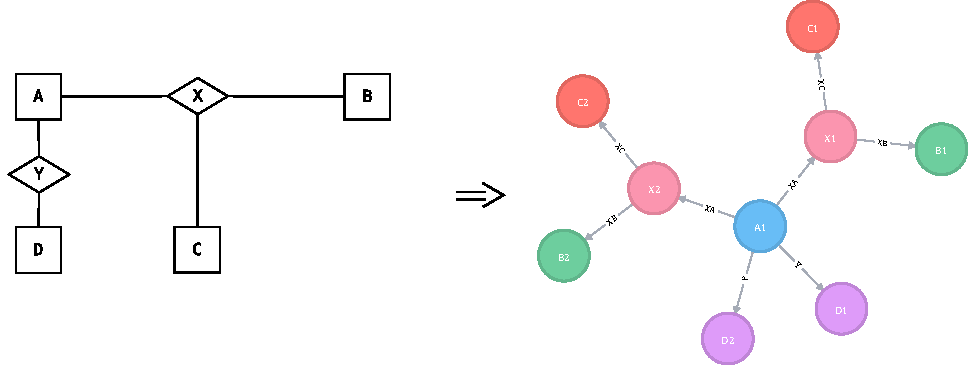
\includegraphics[height=150pt]{resources/er-to-neo4j.pdf}
	\caption{Example conversion of an ER diagram into a \neoj graph}
	
	%Create (a1:A {name: 'A1'}), (b1:B {name: 'B1'}), (b2:B {name: 'B2'}), (c1:C {name: 'C1'}), (c2:C {name: 'C2'}), (d1:D {name: 'D1'}), (d2:D {name: 'D2'}), (x1:X {name: 'X1'}), (x2:X {name: 'X2'}), (a1)-[:XA]->(x1), (x1)-[:XB]->(b1), (x1)-[:XC]->(c1), (a1)-[:Y]->(d1), (a1)-[:Y]->(d2), (a1)-[:XA]->(x2), (x2)-[:XB]->(b2), (x2)-[:XC]->(c2)
	
	\label{fig:example-er-diagram}
\end{figure}

\subsection{\masymos}
\label{sec:background:graph-db:masymos}

This work is mainly based on \masymos, "a graph database for simulation models and associated data" \cite{Henkel2015}, which is implemented using \neoj \todo{add cite to neo4j book}.
As mentioned in Section \ref{sec:graph-db}, models often encode simulation networks, which can easily be represented as graphs, but are inhomogeneous. This proves a representation in a table based relational database to be inefficient and difficult \todo{elaborate}, hence those databases are made to store highly structured information, e.g. numerical data. In conclusion they are less efficient in storing standard encoded models together with links to other data sources (e.g. ontologies), because there is no common schema describing the structure. This results in a conflict between representing this linked data and keeping an efficient database.

Since \masymos is developed for "storing and retrieving structural information of biological models" \cite{Henkel2015}, it needs to incorporate mentioned graph representations of simulation networks and an efficient way to query those. Therefore \neoj was the ideal choice, as it works as large property graph, but also "follows fundamental properties of databases, i.e. the ACID principles. \cite{Henkel2015}

The internal schema used by \masymos is shown in figure \ref{fig:background:graph-db:masymos}, features a \texttt{DOCUMENT} node as standard entry point. It represents the actual \xml document and has only one direct child: The \texttt{MODEL} node, which in contrast is the entry point for the actual model and represents the \xml root node.

Beyond these two nodes, the schema depends on the format, encoding the imported model. For \sbml the \texttt{MODEL} node is linked to compartments, species, and reactions. Which on the other hand are linked among each other, expressions relations like reaction reactants and products, or association to a compartment.
Whereby in \cellml the \texttt{MODEL} node links to components, which again contain variables and mathematical expressions, manipulating other variables.

Further semantic annotations, like ontology terms or publication and author relations, are represented by additional nodes and link to the corresponding ontology term, stored in \neoj, or the interrelated publication or person node. 
Ontology terms are imported according to their hierarchical structure from the \owl representation, which preserves the classification information and therefore allows for searching for abstract terms, but traversing to more detailed ones and vice versa.
Commonly imported ontologies are biomodels-qualifier \footnote{\todo{get link to biomq}}, gene ontology \footnote{\todo{go link}} and \todo{another onto}

In addition to explicit links the graph database backend of \masymos allows to include implicit links into analysis (those with more than one hop in the graph). Implicit links can link between two models, published by the same person or between model with common annotations, or even between models using annotations of the same ontology branch
Further, to allow for easy upwards traversal, all relations also feature a common relation to the next higher node in hierarchy, called \texttt{belongs\_to}.

\todo{paragraph about shortcomings}
\begin{figure}
	\centering
	\includegraphics[height=150pt]{resources/masymos_struc_figure2.eps}
	\caption{Structure representing \sbml and \cellml models in \masymos. Figure taken from Henkel et al., 2015 \cite{Henkel2015}}
	\label{fig:background:graph-db:masymos}
\end{figure}

\begin{comment}
% following some quotes from the Henkel2015 paper
\begin{itemize}
	\item This work is based on MaSyMoS, "a graph database for simulation models and associated data" \cite{Henkel2015}
	\subitem \cite{Henkel2015} Many models in public databases encode networks that can be represented as graphs
	\subitem \cite{Henkel2015} relational databases were developed for homogeneous, structured data, e.g. numerical data
	\subitem \cite{Henkel2015} Designing a relational representation for these links and keeping the database efficient at the same time are impossible
	
	\item \cite{Henkel2015} MaSyMos is a database based on neo4j for storing and retrieving structural information of biological models
	\subitem \cite{Henkel2015} We chose the graph database Neo4J (25)
	\subitem \cite{Henkel2015} follows the fundamental properties of databases, i.e. the ACID principles
	
	\item \cite{Henkel2015} biological models are represented in heterogenous data structures e.g. networks. Traditional relational databases are build to quickly process highly structured data in tables, therefore they are less efficient in storing and retrieving standard encoded models, due to their highly linked structure
	\subitem \cite{Henkel2015} No unified schema exists for models and meta-data, making it difficult to define a relational database schema
	\subitem \cite{Henkel2015} highly linked models, model entities and meta-data are difficult to represent in a table-based relational database
	\item \masymos data model and structure
	\subitem \cite{Henkel2015} document root node is created for each data item
	\subitem each model is represented by a model node
	\subsubitem entry point for each model import is a document node
	\subitem \cite{Henkel2015} Attached to the model node are annotation nodes, including the reference publication
	\subitem in SBML compartments, species and reactions are linked to the model node
	\subitem in CellML each component is linked to the model node, further containing variables and mathematical relationships to manipulate other variables
	\subsubitem \cite{Henkel2015} component contains vari- ables and mathematical relationships that manipulate those variables
	\subitem Experiment setups are stored under a SEDML node, instead of a model node. In comparison to species, reactions, compartments or components the SEDML node has links to Modelreference nodes, as well as nodes pointing to different model entities used in plots. Nevertheless no processing information is stored in the database.
	\subsubitem \cite{Henkel2015} SEDML node serves as the anchor for an experiment
	\subsubitem \cite{Henkel2015} Modelreference node links the experiment to all Model nodes used in the simulation
	\subsubitem \cite{Henkel2015} do not store the specific processing of a model entity
	\subitem Semantic annotations and cross-references from the models are stored as seperate nodes and linked to the ontology node representing the used ontology term.
	\subsubitem \cite{Henkel2015} Semantic annotations and cross-references
	\subsubitem \cite{Henkel2015} We parse these ontologies and add all concepts and relations as nodes and edges, respectively.
	\subitem ensure an easy traversal upwards, a connection is created from each node of the stored model that points to the parent of the current node. The corresponding edges are named belongsTo]
	\item Linking model related data
	\subitem main advantage to prior mentioned storage in relational databases is the possibility to flexibly link data between different domains. //Henkel et al.// describes 3 different links, which are currently implemented: 1. links between (model) annotations and the corresponding ontology term 2. links between models or model entities and SEDML simulation descriptions or respectively SEDML variables 3. links between model entities in different standard format representation
	\subsubitem \cite{Henkel2015} The main advantage of the previously described concept is its possibility to define flexible links between the data do\item mains)
	\subsubitem \cite{Henkel2015} links between annotations (in SBML, CellML and SED-ML) and ontology concepts)
	\subsubitem \cite{Henkel2015} links between models (in SBML or CellML format) and SED-ML
	\subsubitem \cite{Henkel2015} link is that between a model and a simulation description
	\subsubitem \cite{Henkel2015} links between model entities and SED-ML variables
	\subsubitem \cite{Henkel2015} links between model entities from different model rep- resentation formats
	\subitem \cite{Henkel2015} For each annotation in a model we add an explicit link to the data entry in the ref- erenced bio-ontology
	\subitem This link is shared between all models using this annotation, regardless of the format
	\subitem Further to explicit links (one hop in the graph), MaSyMoS is able to determine implicit links between different models. Those can be established over shared resources like a publication, publication author or annotations with common bio-ontologies. Regarding a publications the database may establish connections based on the likelihood of names by Hemming Distance, resulting in a confidence which can be increased, "" if the entities' annotations match
	\subsubitem \cite{Henkel2015} In addition, we determine implicit links between models of different representation formats
	\subsubitem \cite{Henkel2015} If two models share a publication, the systems can infer implicit links between those entities that are equally named
	\item Implementation
	\subitem MaSyMoS is designed to run as both standalone commandline application with embedded neo4j and as an extension to the neo4j server. Latter is controlled by an unmanaged neo4j plugin providing a RESTful json interface.
	\subitem Same interface also cooperates with the retrieval engine Morre, by providing endpoints to query different search indexes.
	
	\item MaSyMoS project structure
	\subitem The MaSyMoS project is divided into 3 different modules: MaSyMoS-core, Morre and a CLI.
	\subitem The core module contains the logic of the database and communicates directly with neo4j. It consists of routines and a Java API to import models, experiments and ontologies. Further it fetches linked information from common bio-ontologies and manages, updates and queries Lucene indexes.
	\subitem The Command Line Interface (CLI) provides a user interface, to easily interact with the API provided by the core module. It's main purpose was to simplify the development process by skipping the deployment step. Instead it is possible to directly interact with and debug MaSyMoS
	\subitem The Morre module is similiar to the CLI, by providing an way to interact with the core. But instead of providing a user interface, Morre is loaded as neo4j unmanaged extension and exposes a RESTful interface, which can be used to query the Lucene indexes or to push and update models to the database.
\end{itemize}
\end{comment}
\todo{Pictures}


	
	\chapter{Conceptual Architecture}
	\section{Overall system architecture and services}
\begin{itemize}
	\item cf. \ref{fig:system-overview}
	\item \todo{highlight the differences between optimal (proposed) infrastructure and the implementation}
\end{itemize}

\begin{figure}[h]
	\centering
	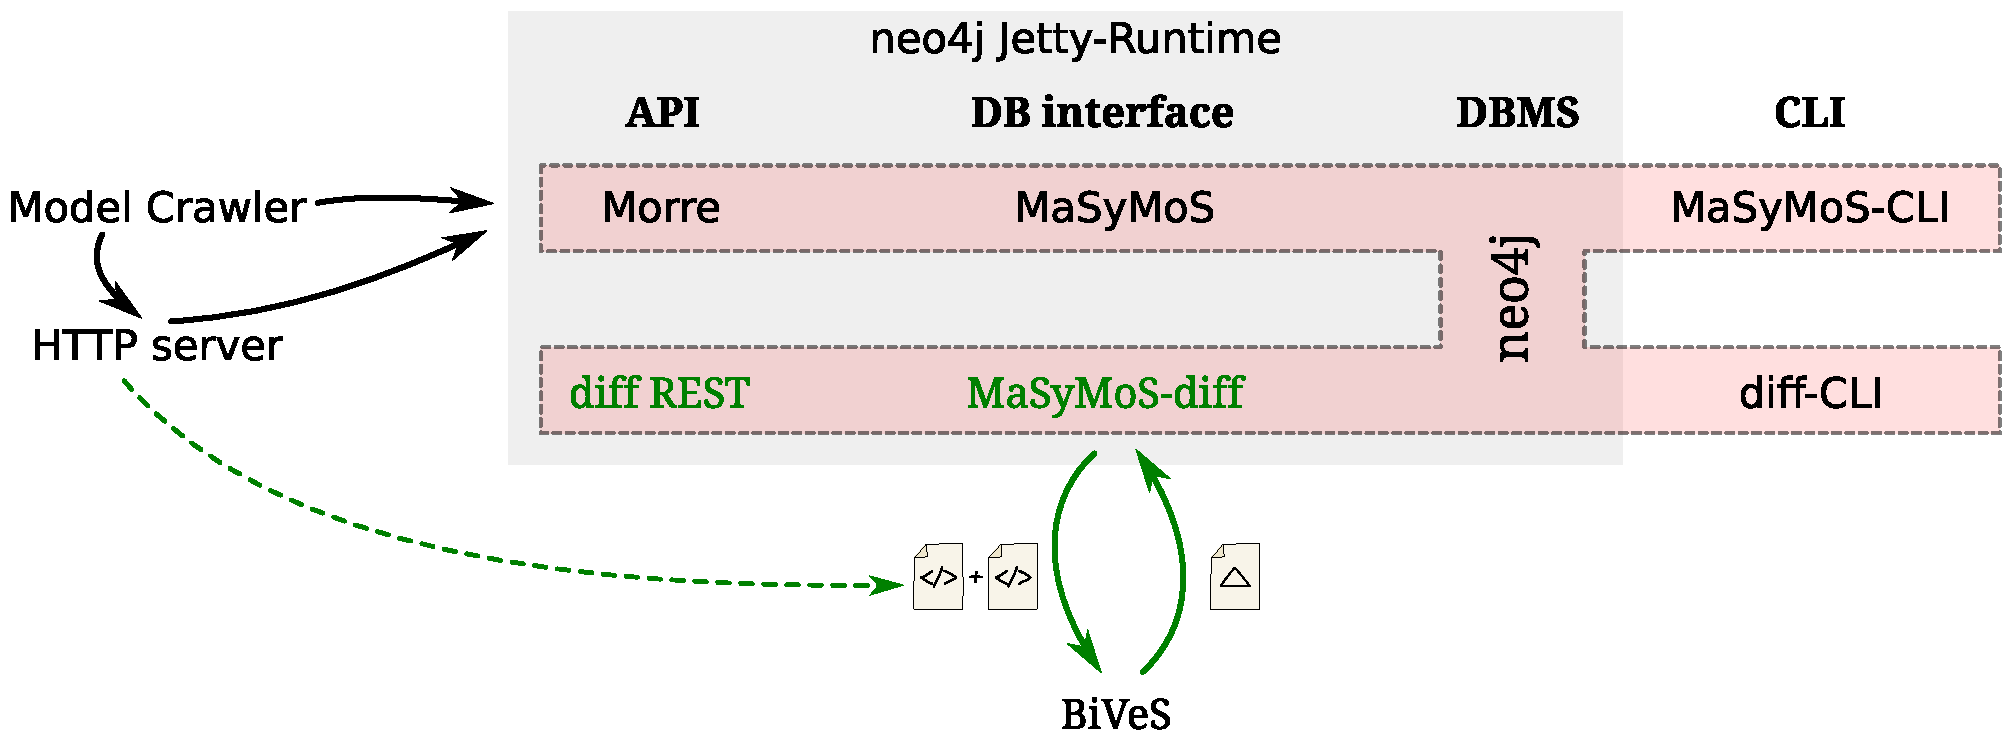
\includegraphics[width=\textwidth]{resources/system-overview-matrix.pdf}
	\caption{Infrastructure overview}
	\label{fig:system-overview}
\end{figure}

\section{Database model and storage decisions}
\begin{itemize}
\item extension to database model cf. \ref{fig:db-model}
	\subitem linking version
	\subitem storing differences
\item decisions on storage model
	\subitem storing each version full (no delta-storage)
	\subitem each version is aware to the search index
	\subitem diff still enables for analysis of changes
	\subitem higher storage consumption
\item extended storage model
\end{itemize}

% description of ER model
Figure \ref{fig:db-er-model} shows the proposed database schema as ER model. To reduce complexity and redundancy, for some entities only classes of higher hierarchy are modeled. E.g. a \texttt{DiffEntry} could be a \texttt{DiffInsert}, \texttt{DiffDelete}, \texttt{DiffModify} or \texttt{DiffMove}. Same applies for \texttt{ModelEntityType} and \texttt{ModelEntity}.
On the left hand side the model shows the existing structure, developed with \masymos. The entities and relations shown on the middle and right hand side shall be added in to process of prototype development.
\todo{Add color to the diagram, to ease explanation}
\todo{Find out, to what a Diff can link}

The schema is build around a \texttt{Diff} entity linking two \texttt{Document} entities, which are representing an (XML-)document containing a model. This entity does not necessarily need to span between two consecutive versions, but I decided for a standard setup it might be less useful to store differences between every possible combination of versions, since it would consume unreasonable amount of storage. Further are diffs concatable, so it does not take any computational effort to generate a diff for larger version steps out of consecutive diffs.

Every \texttt{Diff} entity links to multiple \texttt{DiffEntry} entities via the \texttt{has\_entry} relation. Each \texttt{DiffEntry} represents a difference detected by \bives \cite{Scharm2015}. Not modeled in the ER model is the differentiation between possible types of the diff (insert, delete, move, modify), which will be represented by using different additional label in \neoj.
Each \texttt{DiffEntry} links to at least on \texttt{ModleEntityType} or \texttt{ModelEntity} via either \texttt{old\_entity}, a \texttt{new\_entity}, or both, depending on the type of the difference.
For instance a \texttt{DiffInsert} links to a \texttt{ModelEntityType} or \texttt{ModelEntity} of \emph{Version B} with a \texttt{new\_entity} relation.
In contrast a \texttt{DiffDelete} links to \emph{Version A} with \texttt{old\_entity} to either a \texttt{ModelEntityType} or a \texttt{ModelEntity}. Whereby \texttt{DiffMove} and \texttt{DiffModify} use both relations \texttt{old\_entity} - linking to \emph{Version A} - and \texttt{new\_entity} - linking to Version B.

Additionally a \texttt{DiffEntry} can link to an \texttt{OntologyTerm}, which again can be hierarchical relating to another \texttt{OntologyTerm}. Those terms are taken from the \comodi ontology \cite{Scharm2016}, cf. section \ref{sec:background:comodi}.


\begin{figure}
	\centering
	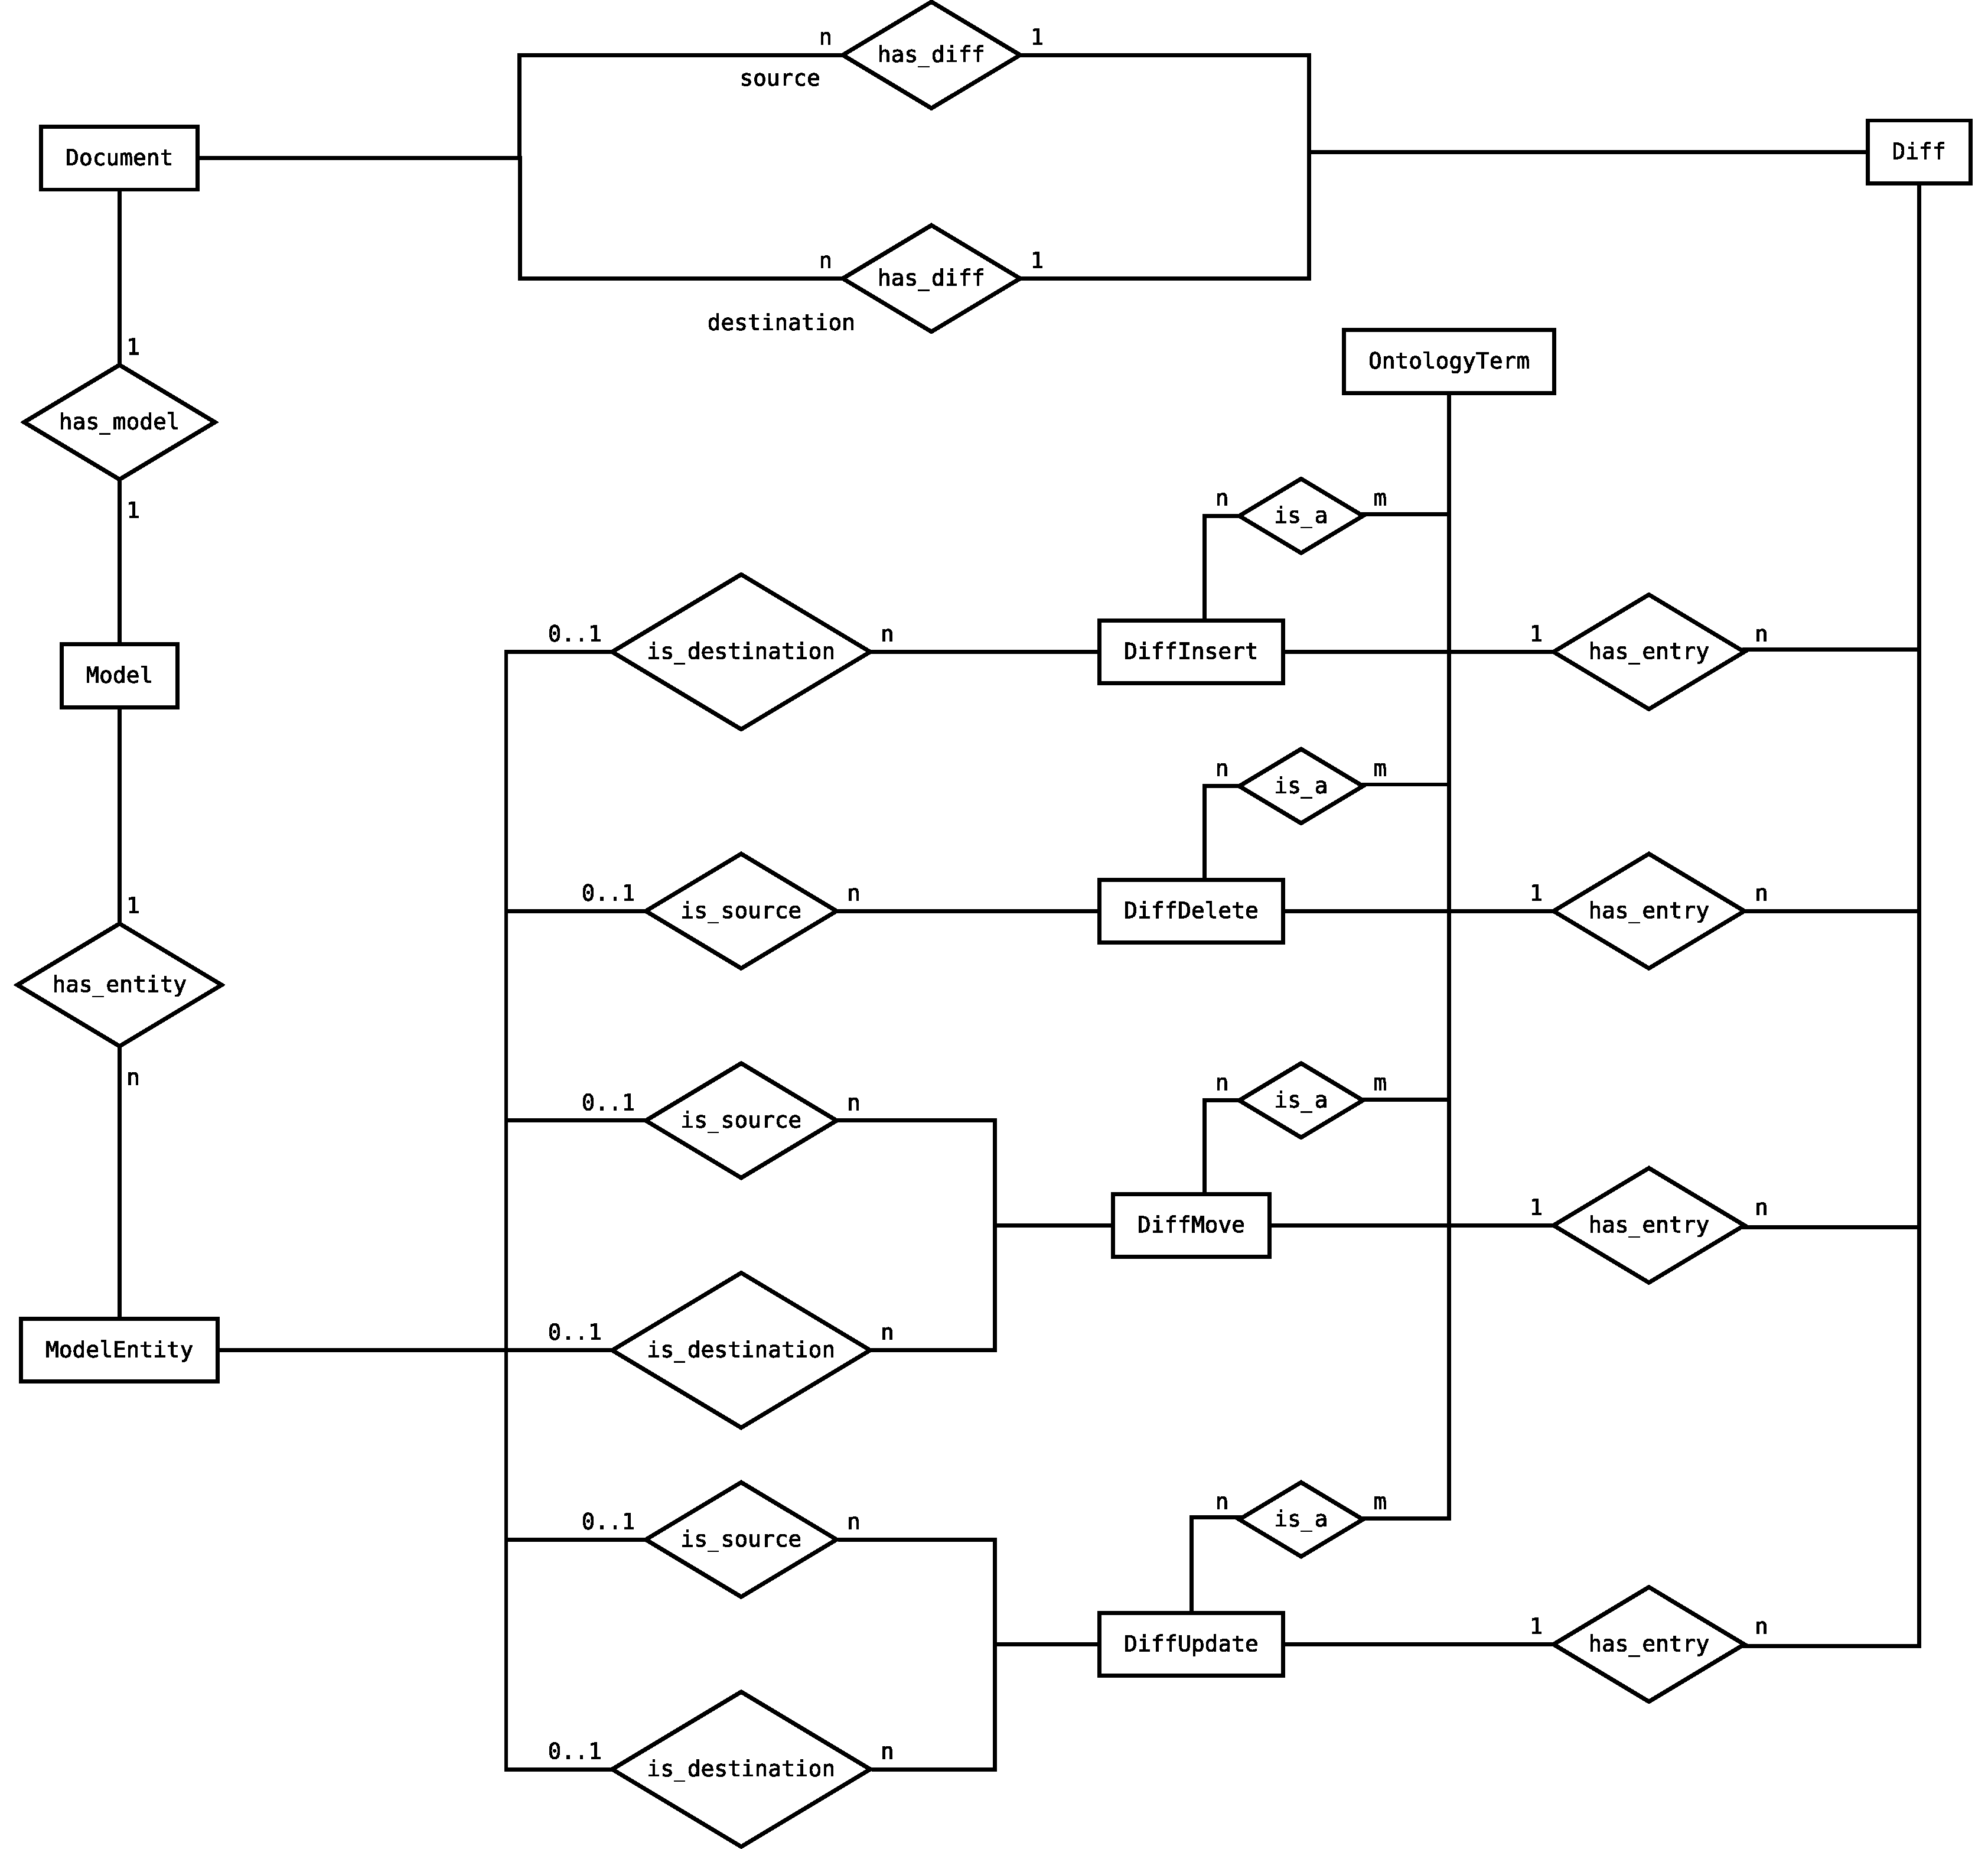
\includegraphics[width=\textwidth]{resources/db-concept-er.pdf}
	\caption{ER model of the proposed database schema}
	\label{fig:db-er-model}
\end{figure}

\begin{figure}[h]
	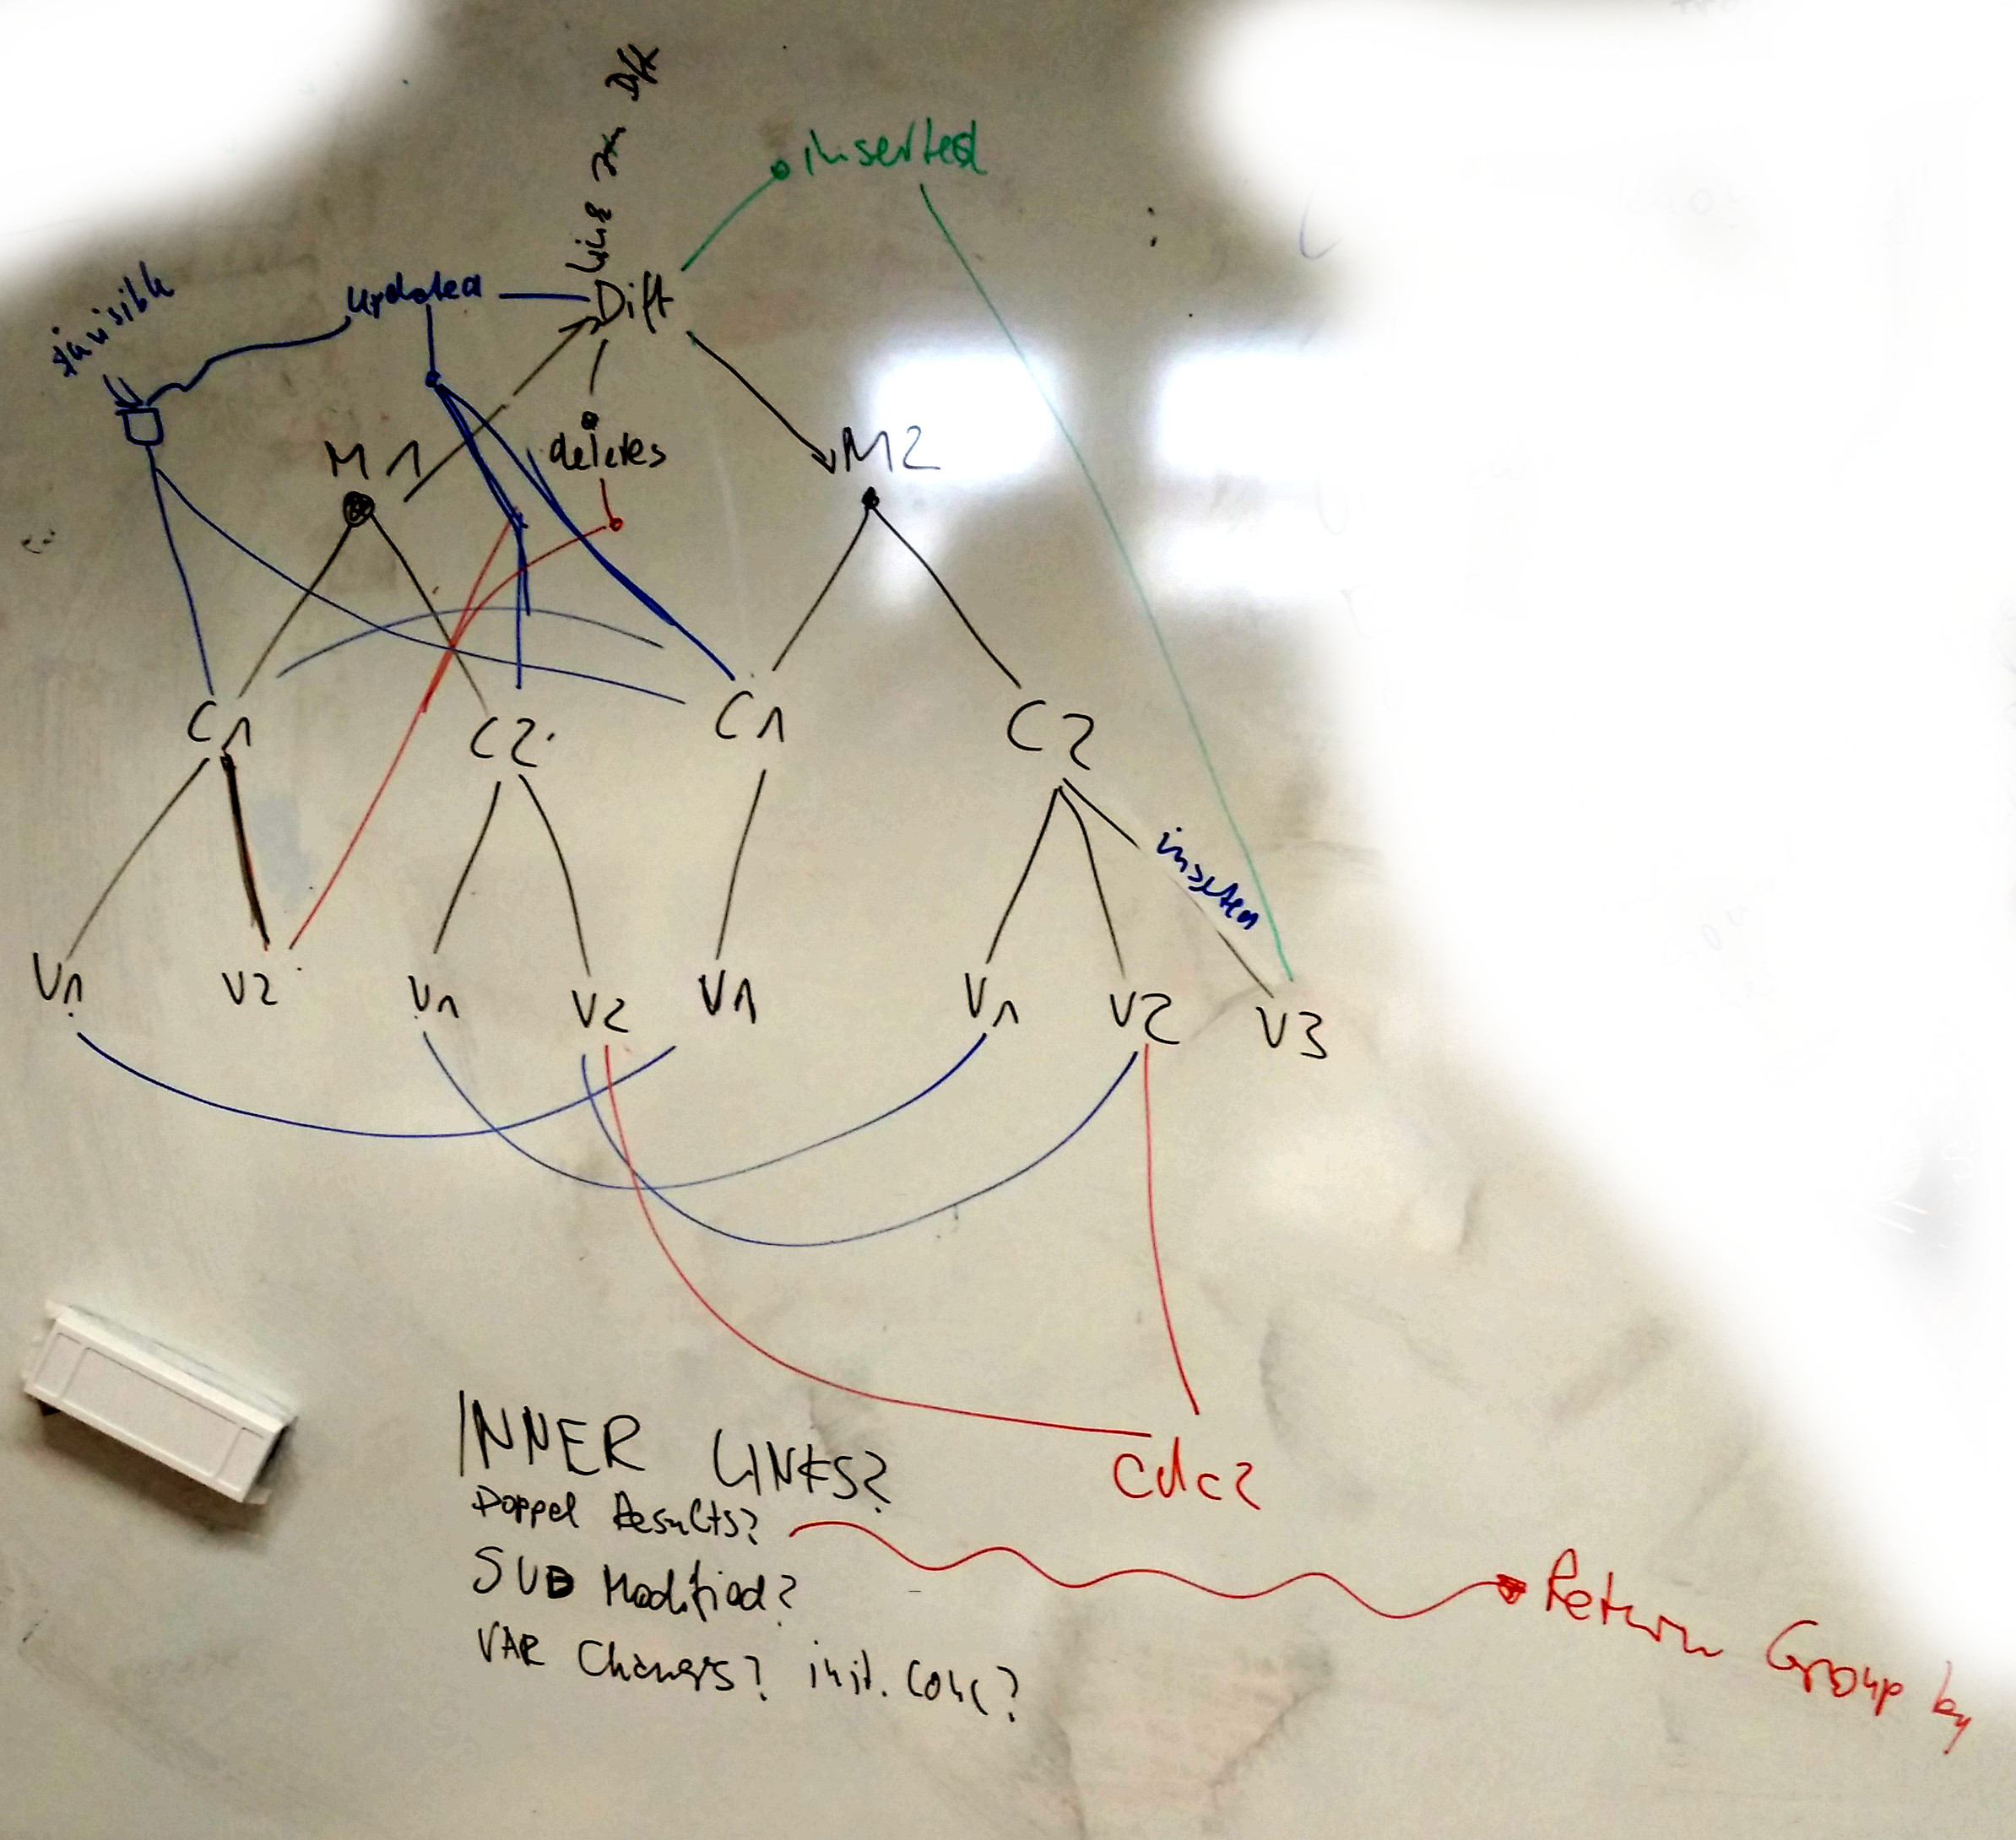
\includegraphics[width=\textwidth]{resources/db_structure.jpg}
	\caption{Proposed database structure}
	\label{fig:db-model}
\end{figure}

	
	\chapter{Results}
	% !TeX spellcheck = en_US
\label{sec:results}

Using the concept, described in Chapter \ref{sec:concept}, I was able to implement the newly designed parts of the ER model, shown in Figure \ref{fig:db-er-model}, in the \masymos \neoj stack. These graph structures are generated by a plugin written to interface the native \neoj API on the one side and \bives on the other.
Converting this formal described ER model into a graph database schema as shown in Figure \ref{fig:results:simple-diff}, was performed as described in Section \ref{sec:background:graph-db:er}. Despite the direct convertibility, some optimizations and adjustments for convenience were made, like introducing the common label \texttt{DIFF\_NODE} for all change types.
Also the figure shows a simplified representation of a delta between two versions of a relatively simple toy model. The figure was reduced to maintain readability, while still illustrating the basic schema.

The schema was designed around a \texttt{DIFF} node, which is linked by \texttt{HAS\_DIFF} relations, from two consecutive versions of the same model. These two versions are again linked with the \texttt{HAS\_SUCCESSOR} and \texttt{HAS\_PREDECESSOR} relations.
The successor and predecessor relations define the version history, whereby the \texttt{DIFF} node clearly indicates the delta between those versions. The \texttt{diffPart} attribute of the \texttt{HAS\_DIFF} relations specifies the direction of the delta, and therefore the role of the participating \texttt{DOCUMENT} nodes. In accordance to the ER model, the role can either be \emph{source} or \emph{destination}.
These terms were chosen, due to their expressiveness in regards to temporal aspects. Otherwise an implication of order, like terms as \emph{old} and \emph{new} suggest, may cause confusion in case of reverse deltas or deltas between completely different models.

However, the central \texttt{DIFF} node links to various changes, using the\linebreak \texttt{HAS\_DIFF\_ENTRY} relation. Since \neoj supports multiple labels per node, the four change types \texttt{DIFF\_INSERT}, \texttt{DIFF\_DELETE}, \texttt{DIFF\_UPDATE}, and \texttt{DIFF\_MOVE} can be grouped together using an additional label \texttt{DIFF\_NODE}. This simplifies queries and will eventually speed them up, because all change types are kept in a single index.
Any kind of \texttt{DIFF\_NODE} might link to any node beneath the \texttt{DOCUMENT} node in at least one of the two compared models, in correspondence to the type of change.
As illustrated by the \texttt{DIFF\_UPDATE} node in Figure \ref{fig:results:simple-diff} (small yellow node, labeled with a \emph{2}). On one hand it connects to the species \emph{A} in the \emph{source} version of the model using the \texttt{IS\_SOURCE} relation. On the other hand it also connects to the updated counterpart in this case species \emph{A} in the \emph{destination} version. It is connected using the \texttt{IS\_DESTINATION} relation.
Furthermore a causality chain among changes is expressed by the \texttt{DIFF\_TRIGGERED\_BY} relation, which points from one \texttt{DIFF\_NODE} to another. This is illustrated by the \texttt{DIFF\_INSERT}, labeled with the number \emph{3}, in Figure \ref{fig:results:simple-diff}. This insert caused four other inserts, describing the insertion of id, name, compartment reference, and initial concentration.

In addition to these structural information each \texttt{DIFF\_NODE} contains all attributes \bives assigns to a change. These \bives specific information include an XPath expressions, name, and id of the changed \xml element. All these attributes can be used together, to locate the change in both versions.
Further the nodes includes the values of \emph{source} and \emph{destination} in case of an attribute change, as well as a possible reference to another change, that triggered this current one.
Besides the \bives attributes, the \texttt{DIFF\_NODE} also contains an \texttt{inherit} flag. It indicates, if a change detected by \bives, does not have a direct match in \masymos's graph structure. Instead the model structure is traversed upwards, until an element is found, which has a representation in the \masymos graph.
This, for instance, applies to changes of a mathematical parameter in a kinetic law of a reaction. In this specific example, the change would be linked to the node representing the reaction, since mathematical structures or kinetic laws are not represented in \masymos. Another example would be text nodes of any kind, which are stored within a Lucene index by \masymos, but not in the graph representation, since they are not an essential part of the models structure.
The \texttt{inherit} flag consequently allows to store and analyze changes, which otherwise could not be integrated into the schema.

Furthermore \texttt{DIFF\_NODE} nodes might link to multiple \comodi terms, whereby \comodi's own relationship names are used, instead of the generic \texttt{is\_a} link, proposed in the concept Section \ref{sec:concept:dbmodel}.
Further \comodi's entire reasoned taxonomy is stored in \masymos, so queries matched against abstract terms also include references to more specialized terms. The resulting network is shown in Appendix \ref{fig:appendix:neo4j-comodi}.
Before generating any deltas the \comodi ontology needs to be imported initially. Otherwise terms might be created on occurrence, but not interlinked according to the taxonomy.
The initial import is performed using already existing mechanisms in \masymos, which were only adjusted, so they can handle dynamic ontology names (cf. Section \ref{sec:impl:masymos}). In this process the ontology is first loaded in its \owl representation and then validated with the Hermit reasoner \citep{Shearer2008}. The second step does not only makes sure that only logically correct ontologies are imported, but also to imports \emph{inferred} ontologies. This moves the logical classification step from querying to the import of ontologies.
A graphical and tabular overview of all used node labels and relation types can be found in Appendix \ref{sec:appendix:meta-map}.

The import of actual models, however, is performed by the \modelcrawler (cf. Section \ref{sec:impl:modelcrawler}), resulting in a \masymos database filled with all model versions of \emph{BioModels Database} and \emph{PMR2} (cf. Section \ref{sec:background:modelrepo}) and a hierarchical file structure containing all original files, complying with the model described in Section \ref{sec:concept:filestorage}.
During a test run from 2016-10-14, this resulted in a dataset with $3367$ distinct models and  $14503$ model versions, with $4.307$ versions per model on average. The accumulated test data consumes $8.5$ GBytes of disc storage for the database, excluding the cached original files (cf. Section \ref{sec:concept:filestorage}).
This data was gathered from all publicly available workspaces in \emph{PMR2} and all releases of the \emph{BioModels database} (cf. Section \ref{sec:background:modelrepo}) using the \modelcrawler (cf. Section \ref{sec:impl:modelcrawler}).
\todo{point to appendix, explaining how the import was done}

On the contrary, models for test purposes and to generate Figure \ref{fig:results:simple-diff} were imported using a small Python\footnote{\url{https://www.python.org/}} script. This script emulates a HTTP daemon, while simultaneously sending import commands to the \masymos \rest interface \morre. It eases the process of importing test data, since neither the \modelcrawler needs to be configure, nor a sane folder structure needs to be built manually.

In conclusion, the extension of the \masymos database allows to store, access, query, and compare multiple versions of biological models, enriched by semantical annotations. Whereas the extended \masymos database is providing an efficient index for a variety of structural, textual and semantic aspects, the original files are still available in the filesystem.
This attempt combines benefits from both approaches.
On one hand the indexed graph database provides excellent analytical features while maintaining reasonable performance. On the other hand it ensures the exact reproduction of the original model files.
Overall this solution meets the requirements set by \citet{Waltemath2013}, that a good "model VCS should be tailored to existing model  representation formats, which are typically XML and RDF based. It should furthermore reflect the temporal evolution of a model and present model changes to the users" \citep{Waltemath2013}.

\begin{figure}[h]
	\centering
	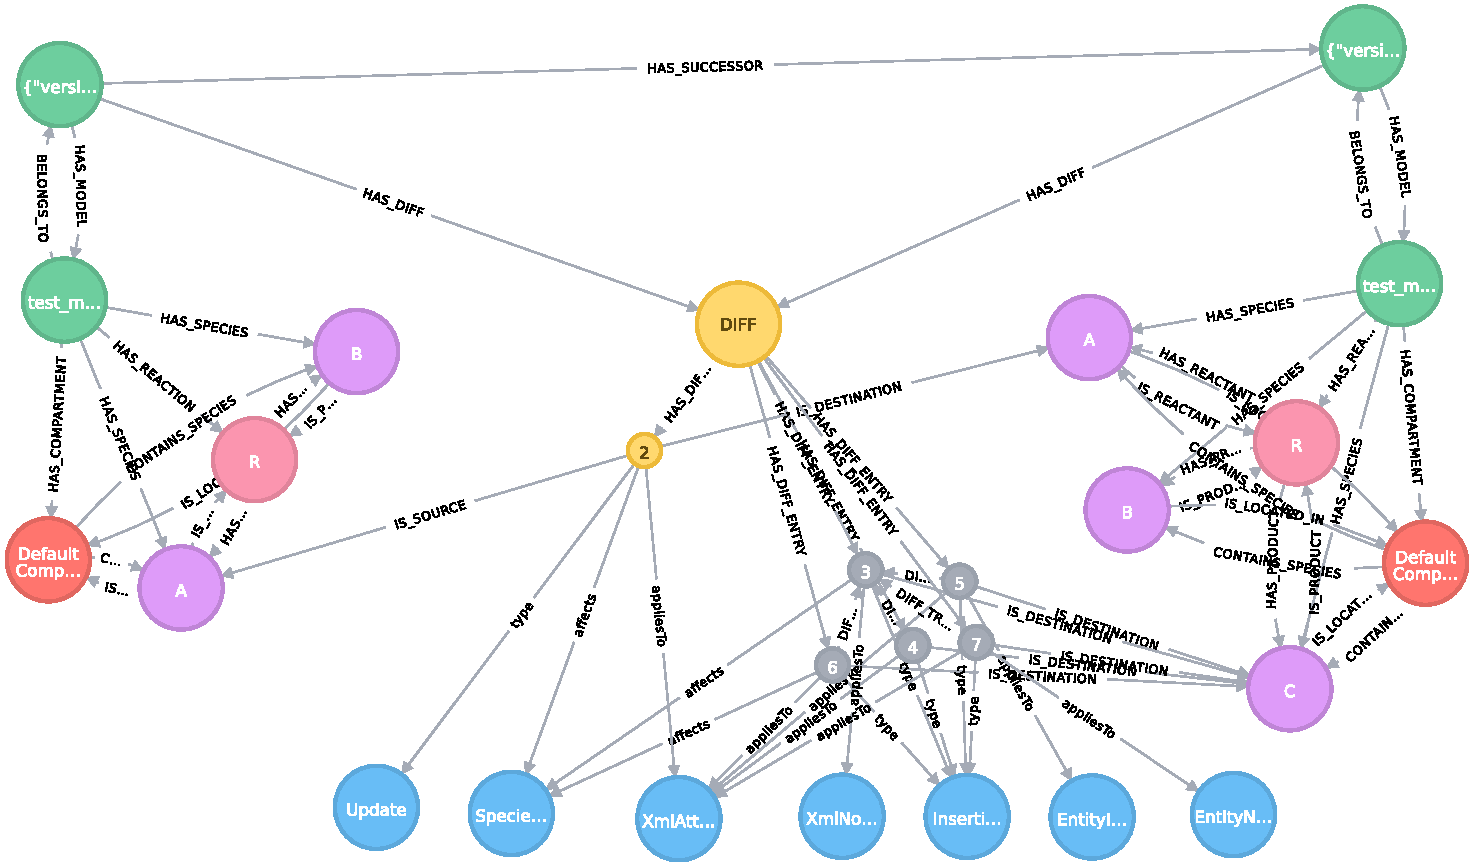
\includegraphics[width=\textwidth]{resources/neo4j-renders/demo-sbml-simple-diff.pdf}
	\caption[Reduced representation of a delta in \masymos, between two versions of a the simple \sbml demo model]{Reduced representation of a delta in \masymos, between two versions of a the simple \sbml demo model. The delta, organized around the \texttt{DIFF} node shows only changes with a direct match in the graph representation. Further most up traversing relations are not shown, to increase readability.
		The small nodes are \texttt{DIFF\_NODE} representing either inserts (green) or a update (yellow) in this example. A full version can be seen in Appendix \ref{fig:appendix:demo-sbml-simple-diff}}
	\label{fig:results:simple-diff}
\end{figure}
 
\begin{comment}
\todo{what's done from the concept}
\todo{still high-level}
\todo{what problem is solved?}

\begin{itemize}
	\item implemented db concept
		\subitem picture from simple-sbml-demo
		\subitem rest of pictures in appendix
	\item Ontology import
		\subitem changes to \masymos core
		\subitem using existing import mechanics, but dynamic
	\item http server storage concept?
\end{itemize}

solved:
"A model VCS should be tailored to existing model representation formats, which are typically XML and RDF based. It should furthermore reflect the temporal evolution of a model and present model changes to the users." \citep{Waltemath2013}

The objective of this thesis is therefore to investigate into a concept to store systems biology models in a way, that multiple versions can be accessed, queried, and compared. Further, semantical annotations of changes between these versions shall be introduced. These additional relations are meant to improve the ability to query for a version of a model by specific criteria and consequently improving the user experience for biologists seeking to build onto existing models, as the evolution of them plays an important role for them \citep{Scharm2015}
\end{comment}
	
	\chapter{Implementation of the Prototype}
	% !TeX spellcheck = en_US
\todo{concrete, low-level stuff}
\todo{what was used, version numbers, etc.}
\todo{pretty short, every subproject gets a section}
\todo{add figure showing differences of concept and implementation, regarding figure \ref{fig:system-overview}}

\section{\modelcrawler}
	\label{sec:impl:modelcrawler}
	The \modelcrawler is not a direct product of this project, but was developed by me in course of my work as student assistant at the department for \sysbio and Bioinformatics. However, it is mentioned here, since it responsible for creating the repository containing all original files, which is one of the integral parts of the presented concept (cf. Section \ref{sec:concept:filestorage}).
	
	The version described here is 0.0.4 mark2, commit \texttt{abb63db}. Overall the function of the \modelcrawler is relatively simplistic and was designed, so it could be ran incrementally, gradually crawling only (a limited amount) new versions. Each pass through therefore consists of two steps: First the databases are crawled, the new versions or releases are downloaded and stored in said file structure.
	Second the \modelcrawler pushes all new model versions to \masymos, theoretically allowing for improved write speed, due to transaction management. However, the main reason for splitting the actions is better error recovery. By keeping the time of write operations on the database short and not running any other concurrent task, the probability of interruptions is minimized. This means, when the \modelcrawler fails, due to bugs in the implementation, changes in the API, or other external influences (e.g. Java Heap Exceptions), the database does not get inconsistent. This is guaranteed, because ahead of inserting data, the \modelcrawler ensures all data is valid and consistent.
	
	However the first step, downloading all new versions, depends heavily on the intended database.
	In case of \emph{BioModels Database} all unknown/new releases are downloaded from the FTP server with Apache Commons Net library version 3.3, unpacked with the Apache Commons Compress version 1.9. Consequently each \xml file is analyzed.
	If a file is already indexed in \masymos, the SHA-1 hash of the files is calculated. If this differs from the file hash of the latest version in \masymos, a new version is assumed. The files are distinguished by their name, which is equivalent to the \emph{BioModels ID}.
	
	This process is easier for \emph{PMR2}, since it already uses git repositories to keep track of versions/revisions of models. Therefore it is just a matter of interfacing the \rest API with Apache HttpClient 4.3 and FasterXMLs Jackson 2.5.1, to list all publicly available repositories. These repositories are then cloned or pulled with eclipses JGit library, version 3.7.0. Following all commits are iterated, and all newer than the latest version in \masymos are considered new.

	Since the \modelcrawler relies on the \masymos database, to identify already existing versions, it can operate stateless between different pass throughs. However, it keeps separately track of already downloaded BioModels releases and all previously cloned git repositories in order to minimize the amount of data, which needs to be transfered.

\section{Extension to the \masymos core}
	\label{sec:impl:masymos}
	\todo{add version number and commit hash}
	The anatomy of the \masymos project is divided into 3 parts: a core, a command line interface, and web \rest interface (cf. Section \ref{sec:background:graph-db:masymos}). This project was designed to mimic this structure, so modifications to the original implementation of \masymos ca be kept minimal. Due to the additive nature of the database concept (cf. Section \ref{sec:concept:dbmodel}), this design constraint could be met, except in one case.
	
	The only direct extension of the core implementation concerns the import of ontologies. By default \masymos allows to load a hard coded set of ontologies, which unfortunately does not include \comodi. Therefore I needed to extend \masymos for this capability. But instead of adding another name to list, I rather implemented a dynamic unique factory. The way \masymos handles ontologies features in particular node label indexes for each ontology, which is used as reverse index to ensure uniqueness of nodes representing a specific term.
	The benefit of this approach is, that even when an ontology is not yet imported, but a model or delta uses certain terms, these are created on demand. Later, when said ontology is loaded, the term representing nodes already exist and can be reused and correctly interconnected.
	The new method I have implemented, now allows to create other dynamic unique factories at runtime, effectively allowing to import any ontology.

	\begin{comment}
	\begin{itemize}
		\item generic ontology import for COMODI
		\item some helper methods/functions
	\end{itemize}
	\end{comment}

\section{\masymos diff plugin}
	\label{sec:impl:diff}
	As mentioned above (cf. Section \ref{sec:impl:masymos}) the implementation structure of this project is meant to mimic the one of \masymos. Hence the main logic is implemented in a core, which possibly gets extended by multiple interfaces (cf. Section \ref{sec:impl:rest}).
	
	This core implementation is designed to operate completely asynchronous, which makes the \texttt{ThreadPoolExecutor} a central part of this implementation. This executor is fed by a priority queue, allowing to prioritize urgent tasks, which may be blocking in terms of user interaction.
	Generally 3 tasks are implemented. First the \texttt{DiffGatherTask}, traverses through the database and submits \texttt{DiffGenerationTask}s for every version hop, not already connected by a delta.
	Secondly the \texttt{DiffGenerationTask} generates the actual delta with \bives and inserts its node representation into the database, using a single transaction.
	Third the \texttt{DiffCleanTask} can be used to remove all existing diffs from the database, which is especially useful during development and testing, but also when \bives is updated, since newer versions might improve detection of  change and annotation of them.
	
	In the current version this implementation uses the \bives library in version 1.9.1. Initially it was planned to rely on the \bives web service, because this is easier to update and would allow for better load balancing in large installations.
	This design decision was changed, because the translation of the \bives \xml output into an interlinked graph representation requires profound knowledge of both compared models. To create a mapping of the XPath expressions from \bives to the actual \xml elements of the model and consequently to nodes in \masymos, the capability of \bives to decode these model files is used. Since the decoding and document tree parsing is also essential for the generation of deltas in \bives (cf. Section \ref{sec:background:diff:bives}), externalizing the delta computation would therefore lead to unnecessary redundant processing and accordingly increase the computation time.
	
	A major issue is occurred in reliability tests of large transactions on the graph database. The origin of this problem lies \neoj's transaction management. Due to the memory consuming nature of graph storage and operations, large transactions may fail, because the Heap Space of the Java Virtual Machine (JVM) was exceeded. Especially the cleaning task suffered from this problem, but also the main \texttt{DiffGenerationTask} did.
	The space consumption of the \texttt{DiffGenerationTask} could be handled by increasing the maximum assigned memory of the JVM. Whereas it was necessary to modify the \texttt{DiffCleanTask} so it uses multiple smaller transaction per pass through.
	
	\begin{comment}
	\begin{itemize}
		\item interaction with \bives and neo4j
		\item problems with Transaction rollback in actually successfull transactions
		\item trigger for generating diffs for new versions
	\end{itemize}
	\end{comment}

\section{\rest interface}
	\label{sec:impl:rest}
	
	To interact with the diff plugin a \rest interface was implemented, similar to \masymos's \morre. It is realized as a unmanaged \neoj extension\footnote{\url{http://neo4j.com/docs/java-reference/current/\#server-unmanaged-extensions}}. As the \neoj manual suggests, it uses JAX-RS\footnote{\url{https://jax-rs-spec.java.net/}} 2.0 to define interfaces and Jackson\footnote{\url{http://wiki.fasterxml.com/JacksonHome}} 2.3.3 to serialize Java objects into \json.
	
	The \rest interface provides 4 endpoints to interact with, either triggering the \texttt{DiffGatherTask} or the \texttt{DiffGenerationTask}, or to enquire some basic statistics of the \texttt{ThreadPoolExecutor} or the database status in terms of generated deltas.
	The thread pool statistics include the number of queued tasks, currently executed tasks, and the immediate running tasks.
	However, the database statistics show the number of \texttt{Diff}s, \texttt{DOCUMENT}s, versions per distinct model, and the distribution of the different types of changes.
	
	\begin{comment}
	\begin{itemize}
		\item \rest interface for requesting diffs
	\end{itemize}
	\end{comment}
	
	\chapter{Discussion}
	\todo{}
\begin{itemize}
	\item Benchmarks/stats on database
		\subitem additional overhead (nodes/relations increase)
	\item How to improve database/reduce overhead
	\item 2 branches of \comodi unused
		\subitem because of automatic generation
		\subitem reason and intention not able to be automatically determined
		\subitem possible extension?
\end{itemize}

	
	%\nocite{*}
	%\bibliographystyle{apalike}
	%\bibliographystyle{apacitep}
	%\bibliographystyle{named}
	%\bibliographystyle{abstract}
	%\bibliographystyle{plainnat}
	\bibliographystyle{abbrvnat}
	%\bibliographystyle{unsrtnat}
	\bibliography{zotero.bib}
	
	\listoffigures
	\begin{appendices}
		\appendixpage
		\noappendicestocpagenum
		\addappheadtotoc
		
		%\chapter*{Appendix}
		% !TeX spellcheck = en_US

% some nice styling for code listings
\definecolor{mygreen}{rgb}{0,0.6,0}
\definecolor{mygray}{rgb}{0.5,0.5,0.5}
\definecolor{mymauve}{rgb}{0.58,0,0.82}

\lstset{ %
	backgroundcolor=\color{white},   % choose the background color; you must add \usepackage{color} or \usepackage{xcolor}
	basicstyle=\footnotesize,        % the size of the fonts that are used for the code
	breakatwhitespace=false,         % sets if automatic breaks should only happen at whitespace
	breaklines=true,                 % sets automatic line breaking
	captionpos=b,                    % sets the caption-position to bottom
	commentstyle=\color{mygreen},    % comment style
	deletekeywords={...},            % if you want to delete keywords from the given language
	escapeinside={\%*}{*)},          % if you want to add LaTeX within your code
	extendedchars=true,              % lets you use non-ASCII characters; for 8-bits encodings only, does not work with UTF-8
	frame=no,	                   % adds a frame around the code
	keepspaces=true,                 % keeps spaces in text, useful for keeping indentation of code (possibly needs columns=flexible)
	keywordstyle=\color{blue},       % keyword style
	language=Octave,                 % the language of the code
	otherkeywords={*,...},           % if you want to add more keywords to the set
	numbers=left,                    % where to put the line-numbers; possible values are (none, left, right)
	numbersep=5pt,                   % how far the line-numbers are from the code
	numberstyle=\tiny\color{mygray}, % the style that is used for the line-numbers
	rulecolor=\color{black},         % if not set, the frame-color may be changed on line-breaks within not-black text (e.g. comments (green here))
	showspaces=false,                % show spaces everywhere adding particular underscores; it overrides 'showstringspaces'
	showstringspaces=false,          % underline spaces within strings only
	showtabs=false,                  % show tabs within strings adding particular underscores
	stepnumber=2,                    % the step between two line-numbers. If it's 1, each line will be numbered
	stringstyle=\color{mymauve},     % string literal style
	tabsize=2,	                   % sets default tabsize to 2 spaces
	title=\lstname                   % show the filename of files included with \lstinputlisting; also try caption instead of title
}

% helper for importing csv files with underscores
\DeclareUrlCommand\UScore{\urlstyle{rm}}
\newcommand{\expUScore}{%
	\expandafter\expandafter\expandafter
	\UScore
	\expandafter\expandafter\expandafter
}

\chapter{Simple demo \sbml models}
\section{Simple demo SBML version1}
\label{sec:appendix:simple-demo:v1}
\lstinputlisting[language=XML]{../supplementary/demo-sbml-simple/version1.xml}

\section{Simple demo SBML version2}
\label{sec:appendix:simple-demo:v2}
\lstinputlisting[language=XML]{../supplementary/demo-sbml-simple/version2.xml}

\chapter{Render of Delta between a more advanced demo model}
\begin{figure}[h]
	\centering
	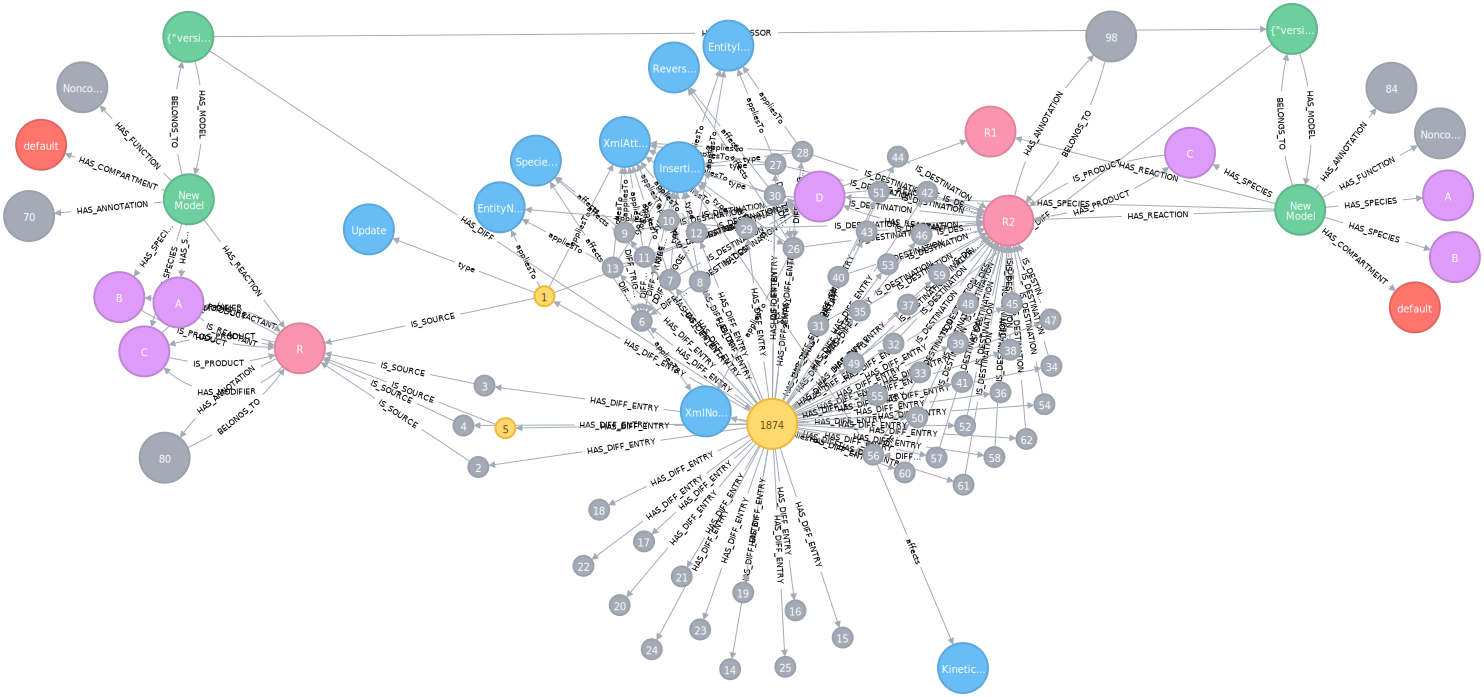
\includegraphics[width=\textwidth]{resources/neo4j-renders/demo-sbml-diff.pdf}
	\caption{\neoj graph representation of a delta between two demo models}
	\label{fig:appendix:demo-sbml-diff}
\end{figure}

\chapter{Representation of \comodi in \masymos}
\begin{figure}[h]
	\centering
	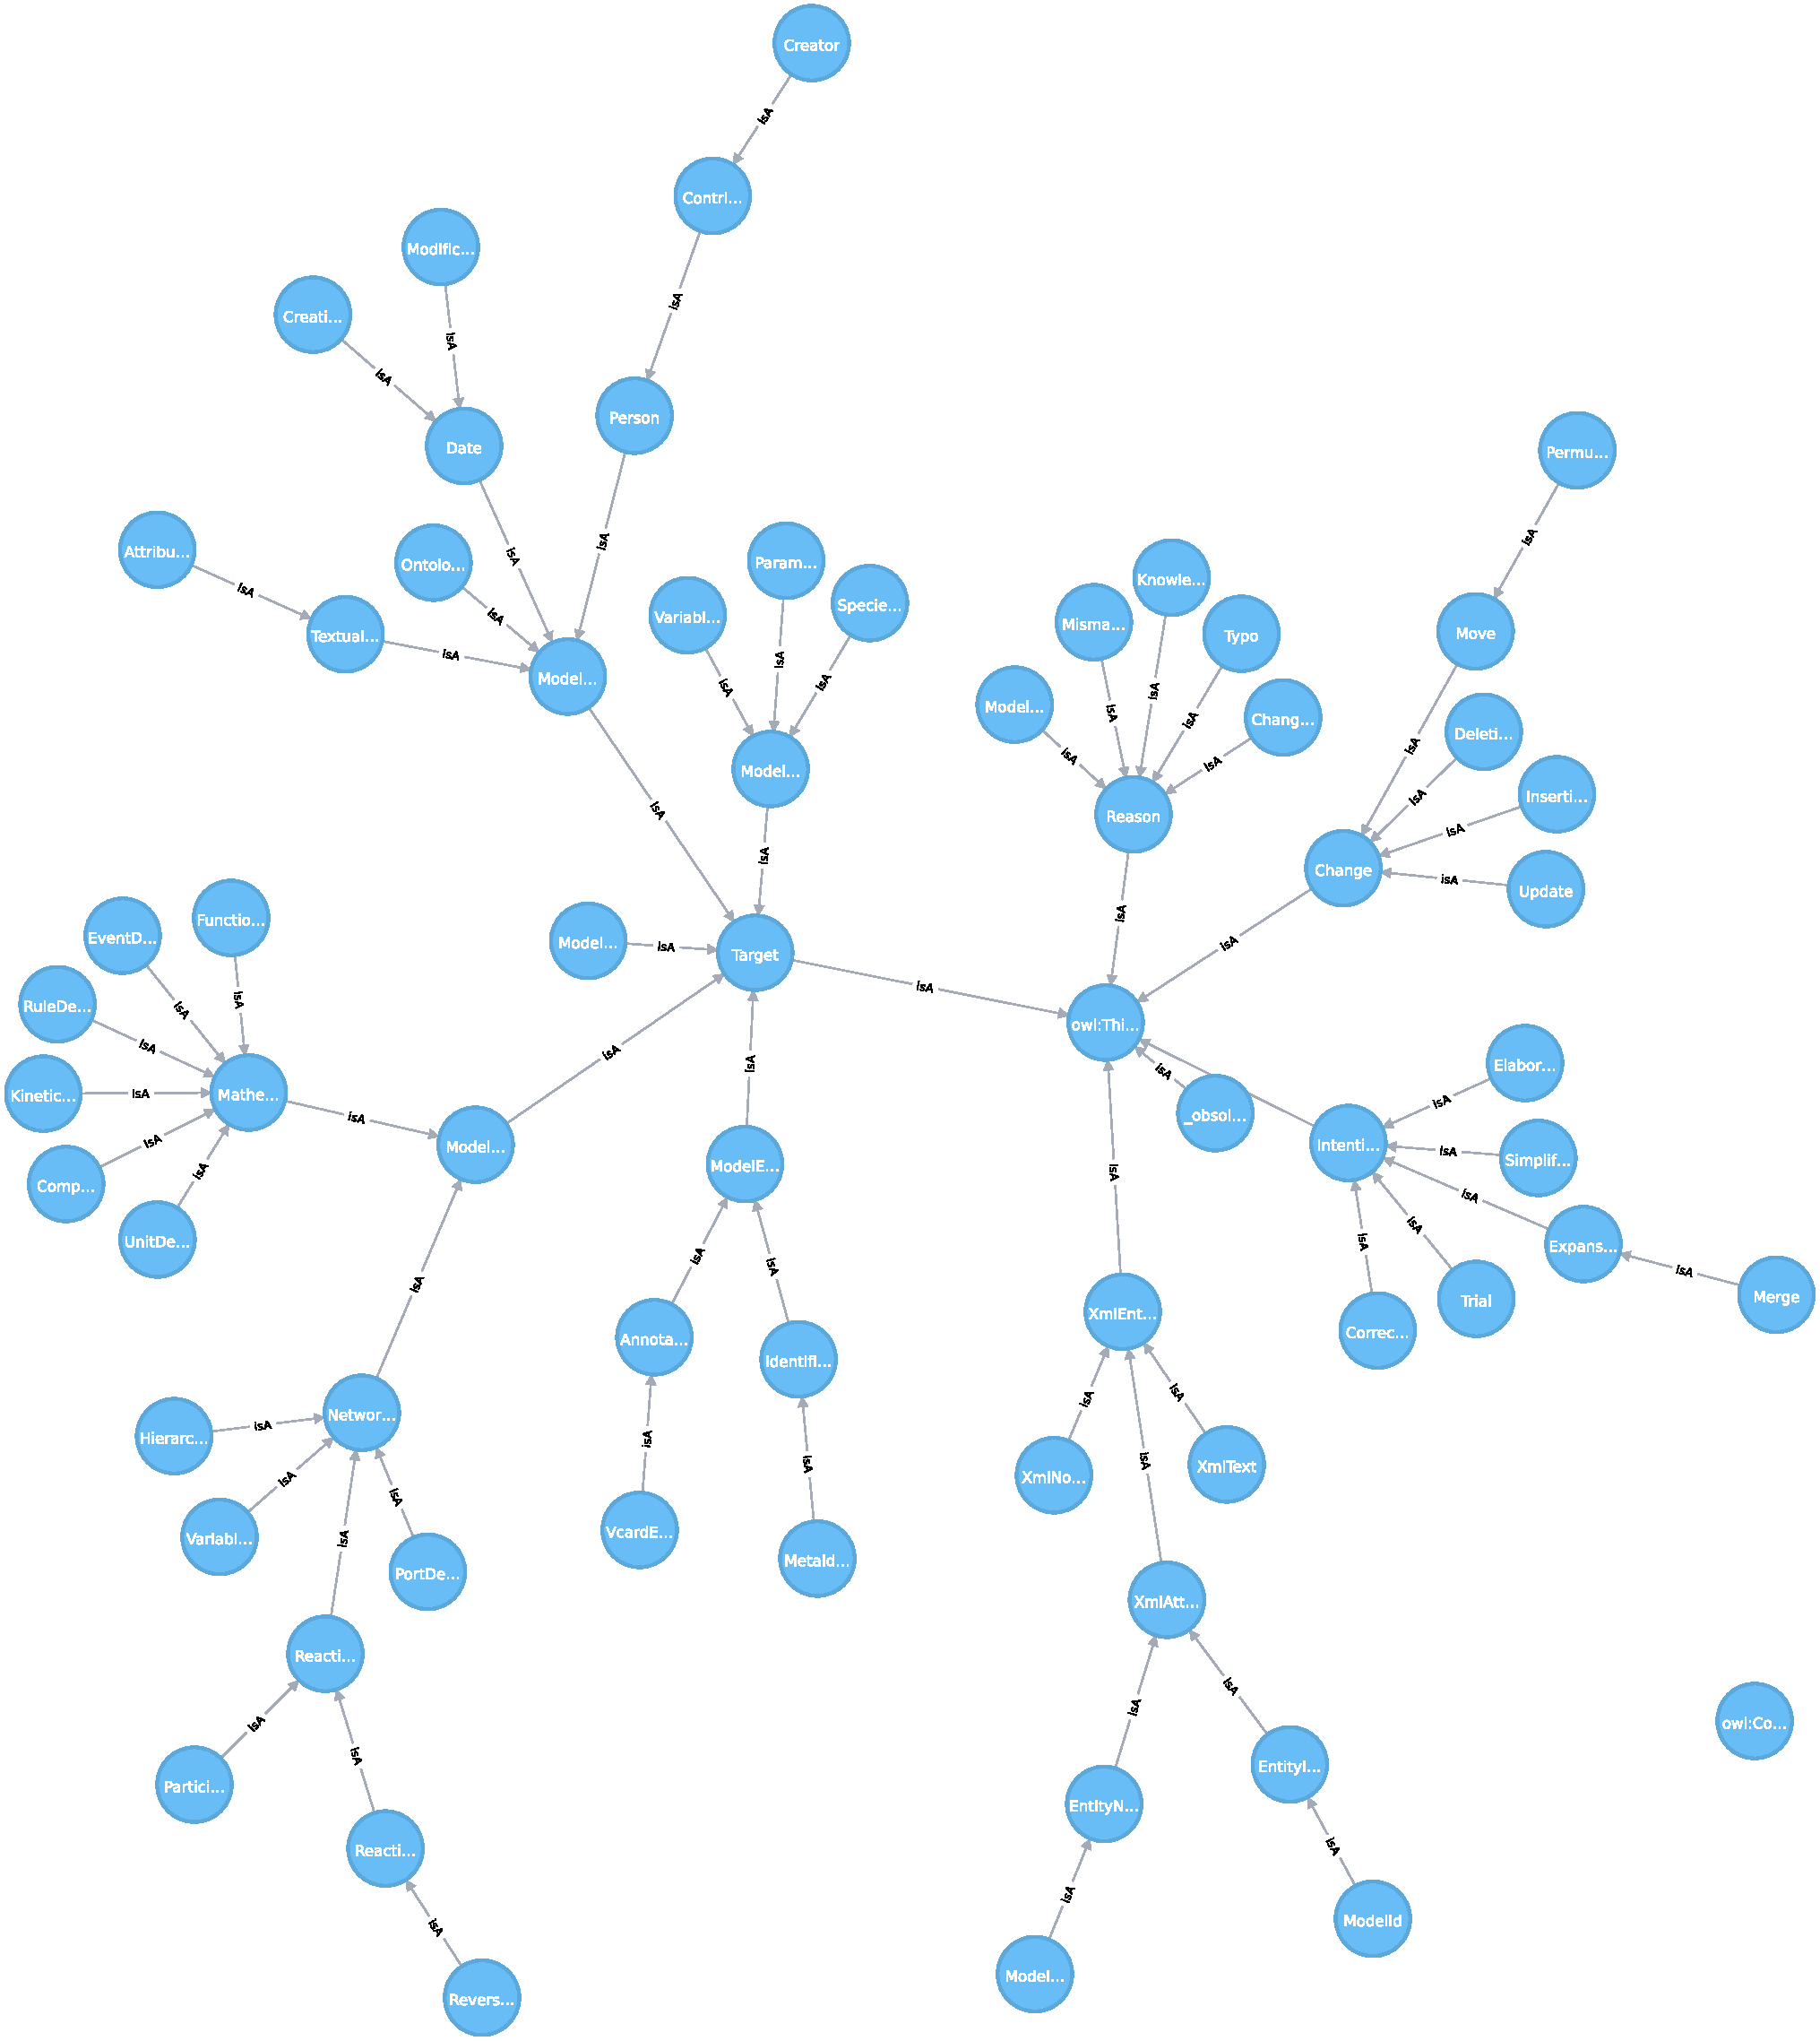
\includegraphics[width=\textwidth,height=0.5\textheight,keepaspectratio]{resources/neo4j-renders/comodi.pdf}
	\caption{Representation of \comodi in \masymos/\neoj}
	\label{fig:appendix:neo4j-comodi}
\end{figure}

\chapter{Overview of Node- and Relationship types}
\todo{tables are ugly as hell...}
\todo{write introduction thingy, where these numbers are coming from}

\section{Graphical Overview}
\begin{figure}[H]
	\centering
	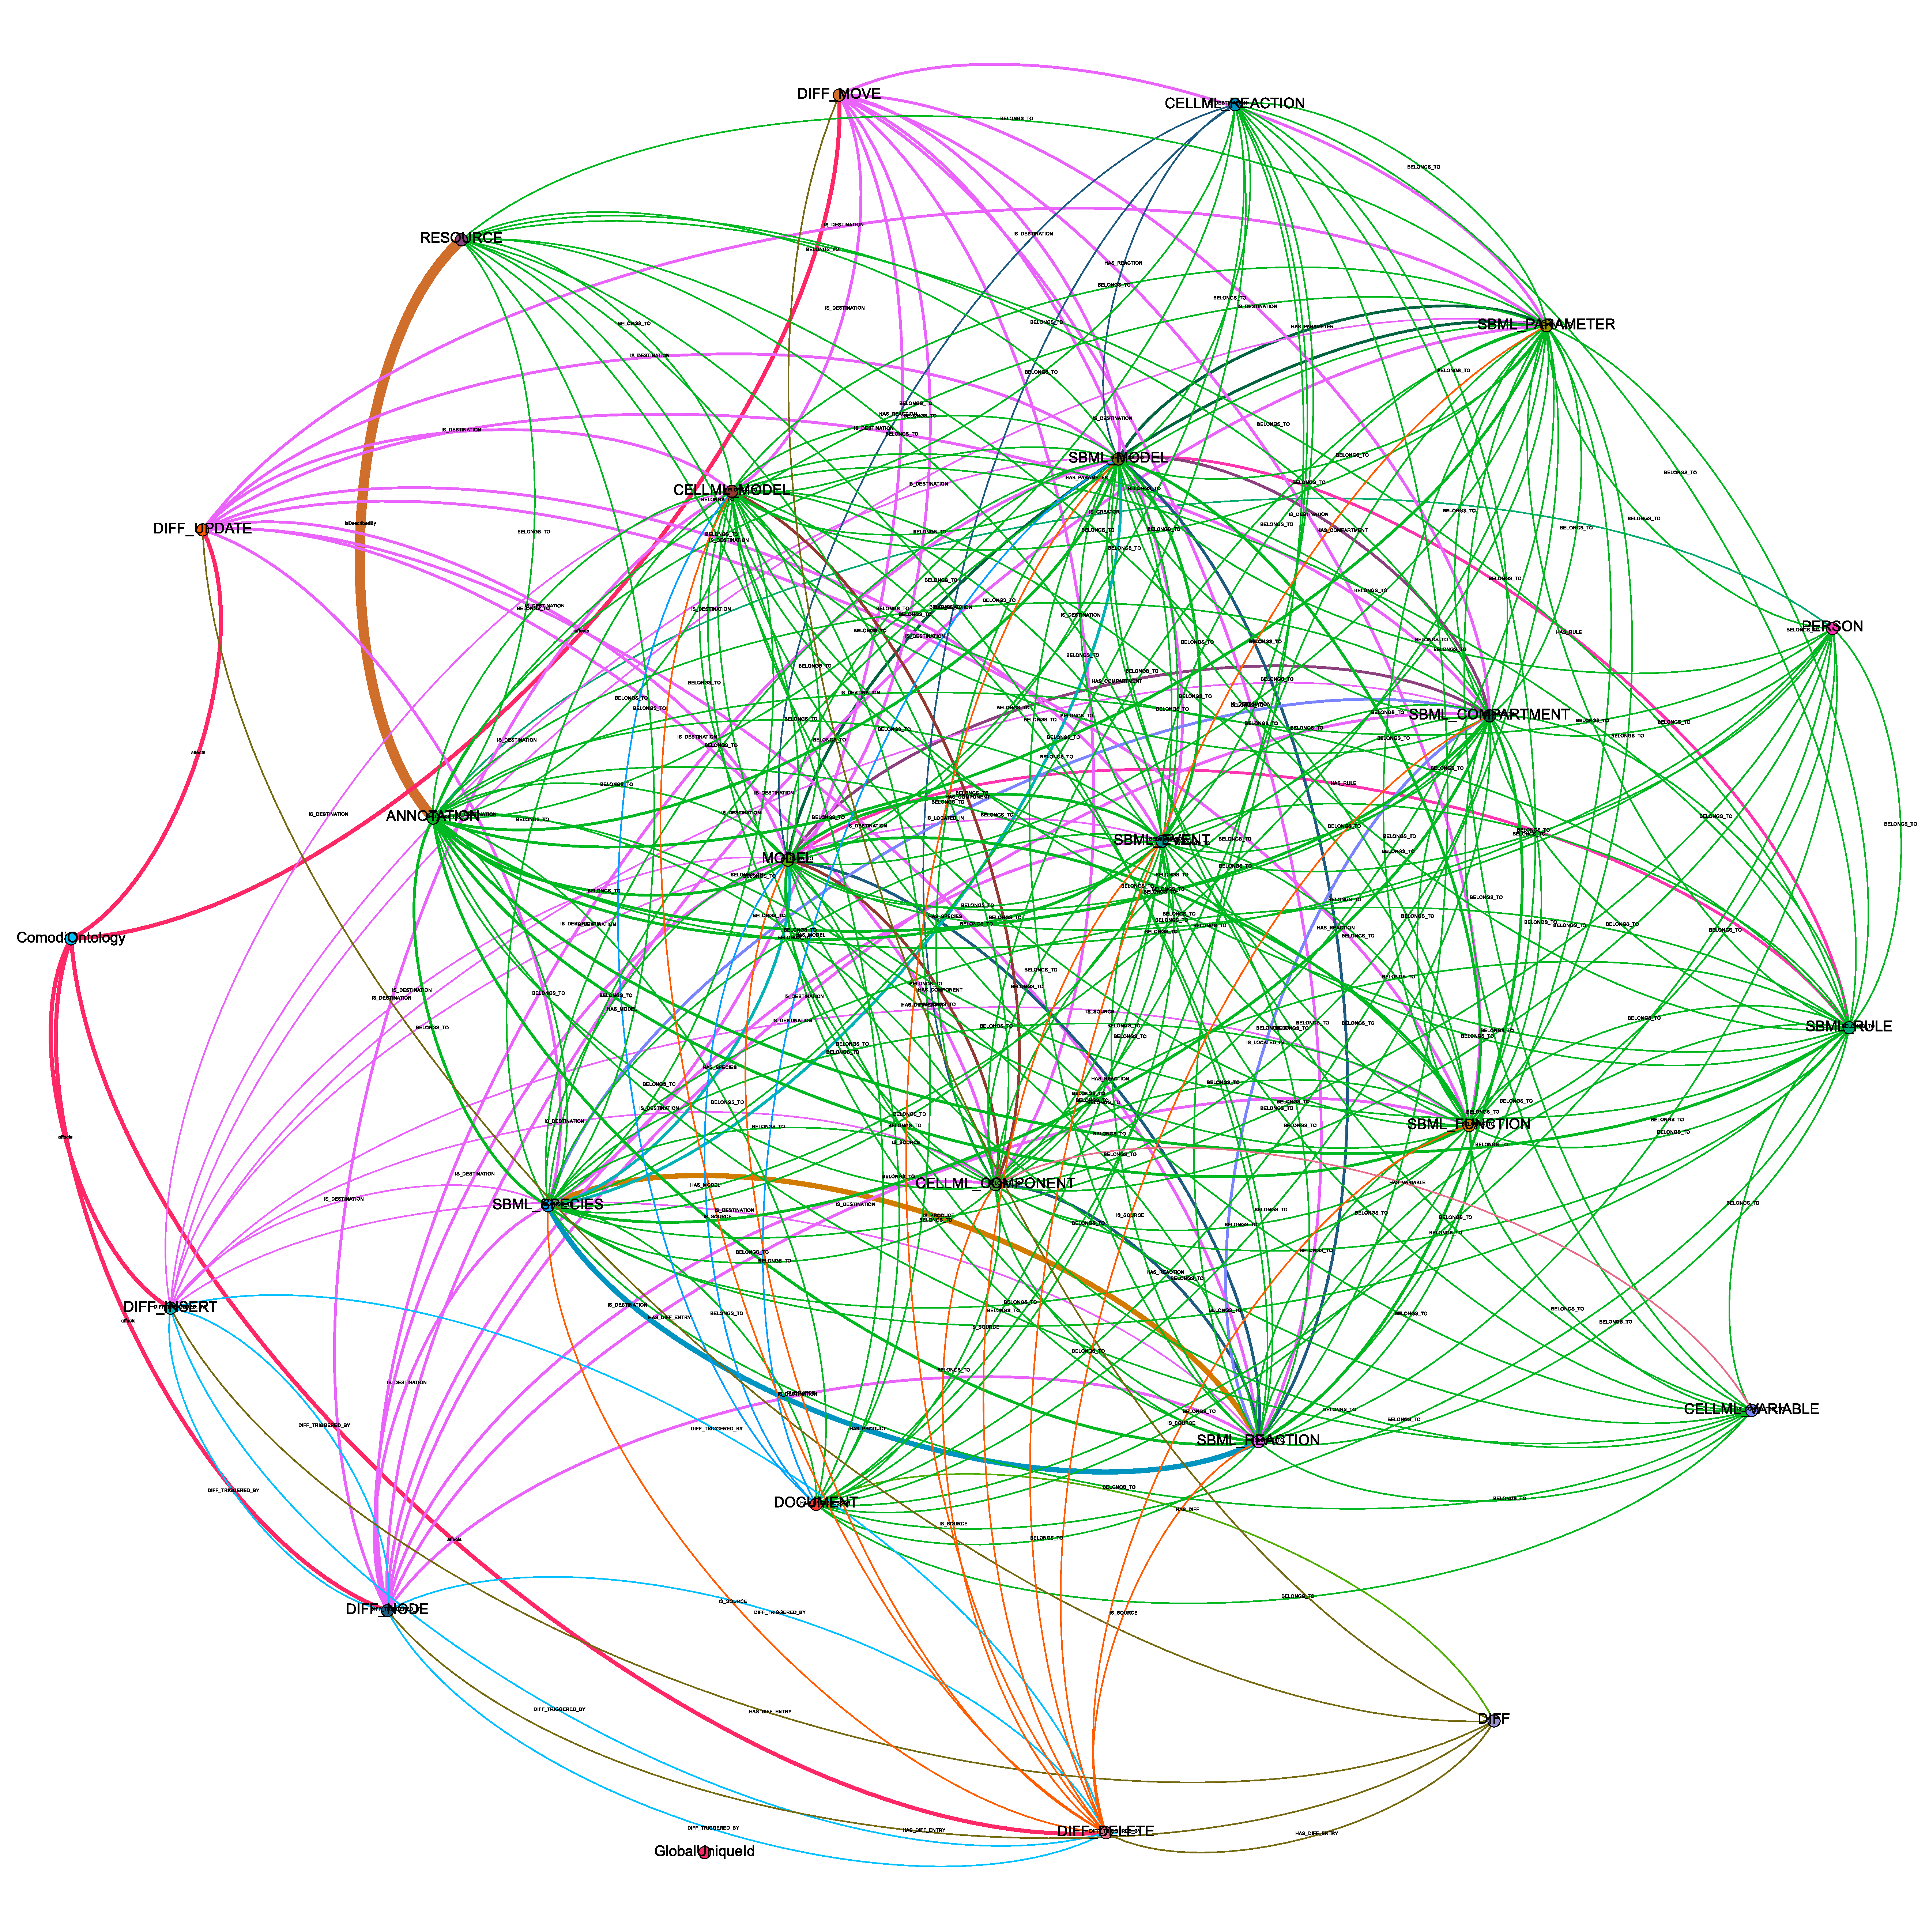
\includegraphics[width=\textwidth,height=0.5\textheight,keepaspectratio]{resources/neo4j-renders/large-test-meta-graph.pdf}
	\caption{Overview of all used node types and relations between them}
	\label{fig:appendix:meta-graph}
\end{figure}

\section{List of all used Node types}
\begin{longtable}{ l r }
	\hline \bfseries Node Label & \bfseries No. of occurrence \\\hline \endhead
	\csvreader[head to column names]{resources/neo4j-renders/large-test-meta-graph-nodes.csv}{} %
	{\expUScore{\label} & \count \\} %
	%\hline
\end{longtable}

\section{List of all used Relationship types}
\begin{longtable}{ l c r r }
	\hline \bfseries Source Node Label & \bfseries Relationship Type & \bfseries Destination Node Label \\\hline \endhead %
	\csvreader[]{resources/neo4j-renders/large-test-meta-graph-edges-expanded.csv}{Source=\sourceNode,Target=\targetNode,label=\relLabel,count=\count} %
	{\expUScore{\sourceNode} & \expUScore{\relLabel} & \expUScore{\targetNode}\\} %
	%\hline
\end{longtable}

	\end{appendices}
\end{document}
